%%%%%%%%%%%%%%%%%%%%%%%%%%%PREAMBLE%%%%%%%%%%%%%%%%%%%%%%%%%%%%%
%%%%%%%%%%%%%%%%%%%%%%%%%%%%%%%%%%%%%%%%%%%%%%%%%%%%%%%%%%
%%			PREAMBLE LATEX GENERAL USE
%%	author: sergio manuel salazar dos santos
%%	email: sergio.salazar.santos@gmail.com
%%	Comment:
%%		Stable, no issues found yet.
%%		Note sequence is importante, and beware of clashing packages.
%%%%%%%%%%%%%%%%%%%%%%%%%%%%%%%%%%%%%%%%%%%%%%%%%%%%%%%%%%
%\documentclass[titlepage, a4paper, 11pt, fleqn, reqno, openany]{report}
\documentclass[titlepage, a4paper, 11pt, reqno, openany]{report}
\usepackage{titlepic}
\usepackage[utf8]{inputenc}
\usepackage[T1]{fontenc}
\usepackage[portuguese]{babel}
%%%%%%%%%%%%%FIXED ORDER%%%%%%%%%FIXED ORDER%%%%%%%%%%%%%%
\usepackage[shortcuts, nopostdot, acronym, toc, nogroupskip, nonumberlist, automake]{glossaries}
\usepackage{scrbase}
\usepackage{babelbib}
%%APPENDIX SETTINGS%%
%\usepackage[title, toc, titletoc, page]{appendix}
\usepackage[toc, page]{appendix}
%%%%%%%%%%%%%%%%%%%%%
\usepackage{verbatim}
\usepackage{url}
\usepackage{listings}
\usepackage[calc, en-US]{datetime2}
\usepackage{etoolbox}
\usepackage{xparse}
%%%%%%%%%%%%%%%%%%%%%%FIXED ORDER END%%%%%%%%%%%%%%%%%%%%%
\usepackage[top=2.5cm,left=3cm,right=2.5cm,bottom=2.5cm]{geometry}
\usepackage[nottoc]{tocbibind}
\usepackage[hidelinks]{hyperref}
\usepackage[usenames, dvipsnames, svgnames, table]{xcolor}
\usepackage{color,colortbl}
\usepackage{graphics}
\usepackage{graphicx}
\usepackage[graphicx]{realboxes}
\usepackage[font=small, labelfont=bf]{caption}
\usepackage{subcaption}
\usepackage{lmodern}
\usepackage{hyphenat}
%%%%%%%%%%%%%%%%%%%%%%%%%%%%%%%%%%%%%%%%%%%%%%%%%%%%%%%%%%
%%%%%%%%%%%%%%%%%%%%%%%%%%%%%%%%%%%%%%%%%%%%%%%%%%%%%%%%%%
\usepackage{multicol}
\usepackage{makecell}
\usepackage{array}
\usepackage{tabularx}
\usepackage[export]{adjustbox}
\usepackage{eurosym}
\usepackage{float}
\usepackage{amsmath}
\usepackage{amsfonts}
\usepackage{amssymb}
\usepackage{mathrsfs}
\usepackage{paralist}
\usepackage{enumerate} %%conflict never put enumitem with enumerate
%\usepackage{enumitem} %%conflict never put enumerate with enumitem
\usepackage{multirow}
\usepackage{lscape}
\usepackage{scrhack}
\usepackage{longtable}
\usepackage{booktabs}
\usepackage[autostyle=true]{csquotes}
\usepackage{calc}
\usepackage{siunitx}
\usepackage{setspace}
\usepackage{lipsum}
\usepackage{moreverb}
\usepackage{rotating}
\usepackage{romannum}
\usepackage{pgfgantt}
\usepackage{tikz}
\usepackage{circuitikz}
\usetikzlibrary{matrix, shapes.geometric, arrows, trees, positioning, calc}
%%%%%%%%%%%%%%%%%%%%%%%%%%%%%%%%%%%%%%%%%%%%%%%%%%%%%%%%%%%%%%%%
\def\mcirc{\mathbin{\scalerel*{\bigcirc}{t}}}
\def\msquare{\mathord{\scalerel*{\Box}{gX}}}
\def\ce{\mathrm{e}}
%%%%%%%%%%%%%%%%%%%%%%%%%%%%%%%%%%%%%%%%%%%%%%%%%%%%%%%%%%%%%%%%
%%BEAMER%%%
%\usetheme{Frankfurt} 
%\usetheme{Boadilla}
%\usetheme{Warsaw}
\makeindex
%%%%%%%%%%%%%%%%%%%%%%%%%%%%%%%%%%%%%%%%%%%%%%%%%%%%%%%%%%%%%%%%
%\bibliographystyle{plain}
\bibliographystyle{ieeetr}
\selectbiblanguage{portuguese}
\setbtxfallbacklanguage{english}
%%%%%%%%%%%%%%%%%%%%%%%%%%%%%%%%%%%%%%%%%%%%%%%%%%%%%%%%%%%%%%%%

%%%%%%%%%%%%%%%%%%%%%%%%%%%%%%%%%%%%%%%%%
%
% DEE@ISEP class for DEE BSc reports
% original file adapted and further developed by Vitor M. R. Cunha
% % v1.3, Apr 2021
%
%%%%%%%%%%%%%%%%%%%%%%%%%%%%%%%%%%%%%%%%%
% original file:
% Masters/Doctoral Thesis 
% Class File
% Version 1.6 (27/8/17)
%
% This class was downloaded from:
% http://www.LaTeXTemplates.com
%
% Authors:
% Vel (vel@latextemplates.com)
% Johannes Böttcher
%
% Notes:
% 1) This class file defines the structure and layout of the template file (main.tex).
% 2) It has been written in such a way that under most circumstances you should not need
% to edit it; updating it to a newer version will be harder. If you do make changes, please change the name of
% the file and add comments to make your changes more visible.
%
% Class license:
% LPPL v1.3c (http://www.latex-project.org/lppl)
%
%%%%%%%%%%%%%%%%%%%%%%%%%%%%%%%%%%%%%%%%%
% sergio santos
% 21-05-2021
% made some changes to fit report style
%%%%%%%%%%%%%%%%%%%%%%%%%%%%%%%%%%%%%%%%%

%----------------------------------------------------------------------------------------
%	CLASS DEFINITION AND PARAMETERS
%----------------------------------------------------------------------------------------

\newbool{portuguese}	%to set the babel language 

\DeclareOption{portuguese}{\booltrue{portuguese}}

\DeclareOption*{\PassOptionsToClass{\CurrentOption}{\baseclass}}
\ProcessOptions\relax

%----------------------------------------------------------------------------------------
%	DEFINE CUSTOM THESIS INFORMATION COMMANDS
%----------------------------------------------------------------------------------------

\NewDocumentCommand{\reporttitle} { o m }{%
	\IfValueTF{#1}{\def\shorttitle{#1}}{\def\shorttitle{#2}}%
	\def\@title{#2}%
	\def\ttitle{#2}%
}
\NewDocumentCommand{\reportsubtitle}{m}{\newcommand{\rsubtitle}{#1}}
\DeclareDocumentCommand{\author}{m}{\newcommand{\authorname}{#1}}
\NewDocumentCommand{\studentnumber}{m}{\newcommand{\stdnumber}{#1}}
\NewDocumentCommand{\studentemail}{m}{\newcommand{\stdemail}{#1}}
\NewDocumentCommand{\advisor}{m m}{\newcommand{\advname}{#1, \url{#2}}}
\NewDocumentCommand{\coadvisor}{m m}{\newcommand{\coadvname}{#1, \url{#2}}}
\NewDocumentCommand{\company}{m}{\newcommand{\companyname}{#1}}
\NewDocumentCommand{\supervisor}{m m}{\newcommand{\supname}{#1, \url{#2}}}
\NewDocumentCommand{\subdate}{m}{\newcommand{\datename}{#1}}
\NewDocumentCommand{\researchgroup}{m}{\newcommand{\groupname}{#1}}

% New command to move content to the next page which prints to the next odd page if twosided mode is active
\newcommand{\checktoopen}{  
	\if@openright\cleardoublepage\else\clearpage\fi
	\ifdef{\phantomsection}{\phantomsection}{}% The \phantomsection command is necessary for hyperref to jump to the correct page
}

\NewDocumentCommand{\bhrule}{}{\typeout{--------------------}}
\NewDocumentCommand{\tttypeout}{m}{\bhrule\typeout{\space #1}\bhrule}

\newcommand{\HRule}{\rule{.9\linewidth}{.6pt}} % New command to make the lines in the title page
\newcommand{\decoRule}{\rule{.8\textwidth}{.4pt}} % New command for a rule to be used under figures
\newcommand{\HRuleFront}{\rule{.98\textwidth}{.3pt}} % New command to make the lines in the title page

\setcounter{tocdepth}{3} % The depth to which the document sections are printed to the table of contents

\ProvideDocumentCommand{\addchaptertocentry}{ m }{%
	\addcontentsline{toc}{chapter}{#1}%
}

\newcommand{\textbetweenrules}[2][.3pt]{%
	\par\vspace{\topsep}
	\noindent\makebox[0.98\textwidth]{%
		\sbox0{#2}%
		\dimen0=.5\dimexpr\ht0+#1\relax
		\dimen2=-.5\dimexpr\ht0-#1\relax
		\leaders\hrule height \dimen0 depth \dimen2\hfill
		\quad #2\quad
		\leaders\hrule height \dimen0 depth \dimen2\hfill
	}\par\nopagebreak\vspace{\topsep}
}

%----------------------------------------------------------------------------------------
%	TITLE PAGES DESIGN
%----------------------------------------------------------------------------------------

\newcommand{\university}{Polit\'{e}cnico do Porto}
\newcommand{\school}{Instituto Superior de Engenharia do Porto}
\newcommand{\department}{Departamento de Engenharia Eletrot\'{e}cnica}
\newcommand{\degree}{Engenheiro Electrot\'{e}cnico}
\newcommand{\frontcourselabel}{}
\newcommand{\aftercourselabel}{}
\newcommand{\degreeacrn}{}

%BSc
\newcommand{\degreetemp}{}
\newcommand{\disclamertemp}{}

\renewcommand{\degreeacrn}{LEEC}
\renewcommand{\degreetemp}{Licenciatura em Engenharia Eletrot\'{e}cnica e de Computadores}
\providecaptionname{english}{\degreetemp}{Degree in Electrical and Computer Engineering}
\providecaptionname{portuguese}{\degreetemp}{Licenciatura em Engenharia Eletrot\'{e}cnica e de Computadores}
\renewcommand{\frontcourselabel}{{\large \degreetemp}\\}
\renewcommand{\disclamertemp}{This report partially satisfies the requirements defined for the Project/Internship course, in the 3\textsuperscript{rd} year, of the }
\providecaptionname{english}{\disclamertemp}{This report partially satisfies the requirements defined for the Project/Internship course, in the 3\textsuperscript{rd} year, of the }
\providecaptionname{portuguese}{\disclamertemp}{Este relat\'{o}rio satisfaz, parcialmente, os requisitos que constam da Ficha de Unidade Curricular de Projeto/Est\'{a}gio, do 3º ano, da }
\renewcommand{\aftercourselabel}{\large \textit{\disclamertemp \degreetemp.}\\}		

%%common
\newcommand{\studentlabel}{Candidate}
\providecaptionname{english}{\studentlabel}{Candidate}
\providecaptionname{portuguese}{\studentlabel}{Candidato}

\newcommand{\nblabel}{nb.}
\providecaptionname{english}{\nblabel}{{No. }}
\providecaptionname{portuguese}{\nblabel}{{Nº }}

\newcommand{\advisorlabel}{Scientific Guidance}
\providecaptionname{english}{\advisorlabel}{Scientific Guidance}
\providecaptionname{portuguese}{\advisorlabel}{Orienta\c{c}\~{a}o Cient\'{i}fica}

\newcommand{\coadvisorlabel}{Scientific Co-Guidance}
\providecaptionname{english}{\coadvisorlabel}{Scientific Co-Guidance}
\providecaptionname{portuguese}{\coadvisorlabel}{Coorienta\c{c}\~{a}o Cient\'{i}fica}

\newcommand{\supervisorlabel}{Advisor}
\providecaptionname{english}{\supervisorlabel}{Advisor}
\providecaptionname{portuguese}{\supervisorlabel}{Orientador}

\newcommand{\companylabel}{Company}
\providecaptionname{english}{\companylabel}{Company}
\providecaptionname{portuguese}{\companylabel}{Empresa}

%%1st page
\newcommand{\printcoverpage}{
	\begin{titlepage}
		\pdfbookmark[0]{Front}{cover}
		\begin{center}
			{\scshape\normalsize \university}\\[3mm]
			{\scshape\LARGE \school}
			\HRuleFront
			\vfill		
			{\huge \bfseries \ttitle\par}\vspace{0.4cm} % Thesis title
			\ifdefined\rsubtitle {\large \bfseries \rsubtitle} \\ \fi 
			% Report sub title, if exists
			\vfill
			{\Large\bf \authorname}\par	
			\vfill
			\textbetweenrules[.3pt]{\degreeacrn}
			\vspace{-8pt}
			\frontcourselabel
			\vfill	
			
\includegraphics[width=6.5cm]{./image/Logo/ISEP_logo.jpg} \\		
			{\scshape\large \department}\\
			{\large \school}\\[1cm]
			\DTMsetdatestyle{mydateformat}
			\ifdefined\datename {\normalsize \datename}\\[5mm] \else {\normalsize \today}\\[5mm] \fi
		\end{center}
	\end{titlepage}
}

%%2nd page
\newcommand{\printaftercoverpage}{
	\checktoopen
	\thispagestyle{empty}
	\begin{center}
		\vspace*{.2\textheight}	
		\aftercourselabel	
		\vfill
		{{\small\bf\studentlabel:} \large \authorname, \nblabel \stdnumber, \url{\stdemail}}\\[4pt]
		{{\small\bf\advisorlabel:} \large \advname }\\[4pt]
		\ifdefined\coadvname {{\small\bf\coadvisorlabel:} \coadvname}\\[4pt] \fi
		\ifdefined\companyname {{\small\bf\companylabel:} \companyname\\{\small\bf\supervisorlabel:} \supname}\\ \fi
		\vfill
		
\includegraphics[width=6.5cm]{./image/Logo/ISEP_logo.jpg} \\		
		{\scshape\large \department}\\
		{\large \school}\\
		{\normalsize Rua Dr. Ant\'{o}nio Bernardino de Almeida, 431, 4200--072 Porto}\\[1cm]
		\DTMsetdatestyle{mydateformat}	
		\ifdefined\datename {\normalsize \datename}\\[5mm] \else {\normalsize \today}\\[5mm] \fi
	\end{center}
}
%%%%%%%%%%%%%%%%%%%%%%%%%%%%%%%%%%%%%%%%%%%%%%%%%%%%%%%%%%

%%%%%%%%%%%%%%%%%%%%%%%%%%%%%%%%%%%%%%%%%%%%%%%%%%%%%%%%%%%%%%%%
\definecolor{light-gray}{gray}{0.95}
\definecolor{lightgray}{rgb}{.9,.9,.9}
%%%%%%%%%%%%%%%%%%%%%%%ISEP SETTINGS START%%%%%%%%%%%%%%%%%%%%%%
\lstset{
	language=C,							% choose the language of the code
	%basicstyle=\small\ttfamily\color{black},
	basicstyle=\footnotesize\ttfamily\color{black},
	keywordstyle=\bfseries\color{blue},
	numbers=left,						% where to put the line-numbers   
	numberstyle=\tiny\color{gray},		% the size of the fonts that are used for the line-numbers
	stepnumber=1,						% the step between two line-numbers. If it's 1 each line will be numbered
	numbersep=2pt,						% how far the line-numbers are from the code
	xleftmargin=2em,					% keep line numbers inside the margins		
	frame=tb,							% frame: top and bottom lines
	framexleftmargin=1.5em,				% frame: adjusts left margin because the xleftmargin numbers setting
	float=!htb,							% if float defined, let Latex manage it
	aboveskip=8mm,
	belowskip=4mm,
	backgroundcolor=\color{light-gray},
	commentstyle=\color{red},			% comment style
	keywordstyle=\color{blue},			% keyword style
	showspaces=false,					% show spaces adding particular underscores
	showstringspaces=false,				% underline spaces within strings
	showtabs=false,						% show tabs within strings adding particular underscores
	tabsize=2,							% sets default tabsize to 2 spaces
	captionpos=b,						% sets the caption-position to bottom
	breaklines=true,					% sets automatic line breaking
	breakatwhitespace=false,			% sets if automatic breaks should only happen at whitespace
	escapeinside={\%*}{*)},				% if you want to add a comment within your code
	morekeywords={*,var,template,new},	% if you want to add more keywords to the set
	stringstyle=\color{orange},
	columns=fullflexible
}
%%%%%%%%%%%%%%%%%%%%%%%%%%%%%%%%%%%%%%%%%%%%%%%%%%%%%%%%%%
%\begin{comment}
\DTMnewdatestyle{mydateformat}{
	\renewcommand{\DTMdisplaydate}[4]{
		    %\DTMshortweekdayname{##4},\space
		\DTMmonthname{##2} \nobreakspace de \nobreakspace
		    %\number##3,\space        
		\number##1                  
	}
	\renewcommand{\DTMDisplaydate}{\DTMdisplaydate}%
}
%\end{comment}
%%%%%%%%%%%%%%%%%%%%%%%ISEP SETTINGS END%%%%%%%%%%%%%%%%%%
\begin{comment}
\setlistdepth{12}
\newlist{enumitem}{enumerate}{12}
\setlist[enumitem,1]{label=\roman*)}
\setlist[enumitem,2]{label=\alph*)}
\setlist[enumitem,3]{label=\arabic*)}
\setlist[enumitem,4]{label=(\roman*)}
\setlist[enumitem,5]{label=(\alph*)}
\setlist[enumitem,6]{label=(\arabic*)}
\setlist[enumitem,7]{label=\roman*)}
\setlist[enumitem,8]{label=\alph*)}
\setlist[enumitem,9]{label=\arabic*)}
\setlist[enumitem,10]{label=(\roman*)}
\setlist[enumitem,11]{label=(\alph*)}
\setlist[enumitem,12]{label=(\arabic*)}
\end{comment}
%%%%%%%%%%%%%%%%%%%%%%%%%%%%%%%%%%%%%%%%%%%%%%%%%%%%%%%%%%
\begin{comment}
\renewcommand{\labelitemi}{$\bullet$}
\renewcommand{\labelitemii}{$\cdot$}
\renewcommand{\labelitemiii}{$\diamond$}
\renewcommand{\labelitemiv}{$\ast$}
\end{comment}
%%%%%%%%%%%%%%%%%%%%%%%%%%%%%%%%%%%%%%%%%%%%%%%%%%%%%%%%%%
\begin{comment}
\tikzstyle{RECTANGLE_2} = [rectangle, draw, text width=5em, text centered, rounded corners, minimum height=4em]
\tikzstyle{RECTANGLE_3} = [rectangle, rounded corners, minimum width=3cm, minimum height=1cm,text centered, draw=black, fill=red!80]
\tikzstyle{RECTANGLE_4} = [rectangle, draw, fill=blue!20, text width=3cm, text centered, minimum height=4em]
\tikzstyle{RECTANGLE_5} = [rectangle, minimum width=3cm, minimum height=1cm, text centered, text width=3cm]
\tikzstyle{RECTANGLE_6} = [rectangle, draw, fill=blue!20, text width=5em, text centered, rounded corners, minimum height=4em]
\tikzstyle{RECTANGLE_7} = [rectangle, draw, fill=blue!20, text width=5em, text centered, rounded corners, minimum height=4em]
\tikzstyle{RECTANGLE_8} = [rectangle, draw, align=left, fill=blue!20]
\tikzstyle{RECTANGLE_1} = [rectangle, rounded corners, minimum width=1cm, minimum height=1cm,text centered, draw=black, fill=green!%30]
\tikzstyle{DIAMOND_1} = [diamond, draw, fill=blue!20, text width=4.5em, text badly centered, node distance=4cm, inner sep=0pt]
\tikzstyle{DIAMOND_2} = [diamond, minimum width=3cm, minimum height=1cm, text centered, draw=black, fill=green!30]
\tikzstyle{DIAMOND_3} = [diamond, draw, text width=4.5em, text badly centered, node distance=3cm, inner sep=0pt]
\tikzstyle{DIAMOND_4} = [diamond, draw, fill=blue!20, text width=4.5em, text badly centered, node distance=3cm, inner sep=0pt]
\tikzstyle{DIAMOND_5} = [diamond, draw, fill=blue!20, text width=4.5em, text badly centered, node distance=3cm, inner sep=0pt]
\tikzstyle{DIAMOND_6} = [diamond, draw, fill=blue!20, text width=4.5em, text badly centered, node distance=4cm, inner sep=0pt]
\tikzstyle{DIAMOND_7} = [diamond, draw, align=left, fill=blue!20]
\tikzstyle{ELLIPSE_1} = [draw, ellipse,fill=red!20, node distance=3cm, minimum height=2em]
\tikzstyle{ELLIPSE_2} = [draw, ellipse,fill=red!20, node distance=3cm, minimum height=2em]
\tikzstyle{ELLIPSE} = [draw, ellipse,fill=red!20, node distance=3cm, minimum height=2em]
\tikzstyle{TRAPEZIUM_1} = [trapezium,trapezium left angle=70,trapezium right angle=-70,minimum height=0.6cm, draw, fill=blue!20, text width=4.5em, text badly centered, node distance=3cm, inner sep=0pt]
\tikzstyle{TRAPEZIUM_2} = [trapezium, trapezium left angle=70, trapezium right angle=110, minimum width=3cm, minimum height=1cm, text centered, draw=black, fill=blue!30]
\tikzstyle{TRAPEZIUM_3} = [trapezium,trapezium left angle=70,trapezium right angle=-70,minimum height=0.6cm, draw, fill=blue!20, text width=4.5em, text badly centered, node distance=3cm, inner sep=0pt]
\tikzstyle{ARROW} = [thick,->,>=stealth]
\tikzstyle{LINE} = [draw, -latex']
\tikzstyle{MYLINE} = [draw, ->,  thick, shorten <=4pt, shorten >=4pt]
\tikzstyle{TEXT_1}=[draw,text centered,minimum size=6em,text width=5.25cm,text height=0.34cm]
\tikzstyle{TEXT_2}=[draw,text centered,minimum size=2em,text width=2.75cm,text height=0.34cm]
\tikzstyle{TEXT_3}=[draw,minimum size=2.5em,text centered,text width=3.5cm]
\tikzstyle{TEXT_4}=[draw,minimum size=3em,text centered,text width=6.cm]
\tikzstyle{CIRCLE_1}=[draw,shape=circle,inner sep=2pt,text centered, node distance=3.5cm]
\tikzstyle{CIRCLE_2}=[draw,shape=circle,inner sep=4pt,text centered, node distance=3.cm]
\end{comment}
\begin{comment}
%%%%%%%GANTT 1%%%%%%%
\newganttchartelement*{mymilestone}{
	mymilestone/.style={
		shape=isosceles triangle,
		inner sep=0pt,
		draw=cyan,
		top color=white,
		bottom color=cyan!50
	},
	mymilestone incomplete/.style={
		/pgfgantt/mymilestone,
		draw=yellow,
		bottom color=yellow!50
	},
	mymilestone label font=\slshape,
	mymilestone left shift=0pt,
	mymilestone right shift=0pt
}
\newgantttimeslotformat{stardate}{%
	\def\decomposestardate##1.##2\relax{%
		\def\stardateyear{##1}\def\stardateday{##2}%
	}%
	\decomposestardate#1\relax%
	\pgfcalendardatetojulian{\stardateyear-01-01}{#2}%
	\advance#2 by-1\relax%
	\advance#2 by\stardateday\relax%
}
%%%%%%%GANTT 2%%%%%%%
\end{comment}
%%%%%%%%%%%%%%%%%%%%%%%%%%%%%%%%%%%%%%%%%%%%%%%%%%%%%%%%%%
%%%%%%%%%%%%%%%%%%%%%%%%%%%%%%%%%%%%%%%%%%%%%%%%%%%%%%%%%%
\addto{\captionsportuguese}{\renewcommand*\contentsname{\'{I}ndice}}
\addto{\captionsportuguese}{\renewcommand*\lstlistingname{Listagen}}
\addto{\captionsportuguese}{\renewcommand*\lstlistlistingname{Listagens}}
\addto{\captionsportuguese}{\renewcommand*\acronymname{Acrónimos}}
\addto{\captionsportuguese}{\renewcommand{\bibname}{Refer\^{e}ncias}}
\addto{\captionsportuguese}{\renewcommand{\appendixname}{Anexo}}
\addto{\captionsportuguese}{\renewcommand{\appendixpagename}{Anexos}}
\addto{\captionsportuguese}{\renewcommand{\appendixtocname}{Anexos}}
%\noappendicestocpagenum
%%%%%%%%%%%%%%%%%%%%%%%%%%%%%%%%%%%%%%%%%%%%%%%%%%%%%%%%%%
\newtheorem{theorem}{Theorem}
\newtheorem{lemma}{Lemma}
\newtheorem{definition}{Defini\c{c}\~{a}o}
\newtheorem{notation}{Notation}
%%%%%%%%%%%%%%%%%%%%%%%%%%%%%%%%%%%%%%%%%%%%%%%%%%%%%%%%%%
\makeatletter
\renewcommand{\@makechapterhead}[1]{%
	\vspace*{50 pt}%
	{\setlength{\parindent}{0pt} \raggedright \normalfont
		\bfseries\Huge\thechapter.\ #1
		\par\nobreak\vspace{40 pt}}}
\makeatother
%%%%%%%%%%%%%%%%%%%%%%%%%%%%%%%%%%%%%%%%%%%%%%%%%%%%%%%%%%
%\renewcommand\thesection{\arabic{section}}
%\renewcommand\thesubsection{\thesection.\arabic{subsection}}
%%%%%%%%%%%%%%%%%%%%%%%%%%%%%%%%%%%%%%%%%%%%%%%%%%%%%%%%%%
\newcommand{\minipagespace}[1]{{\newline \vspace{#1cm} \newline}}
\newcommand{\tablespace}[1]{{\vspace{#1cm}}}
\newcommand{\figurespace}[1]{{\vspace{#1cm}}}
\newcommand{\listingspace}[1]{{\vspace{#1cm}}}
%%%%%%%%%%%%%FIX SECTION NUMBERING IN CASE REPORT%%%%%%%%%
%\renewcommand\thesection{\arabic{section}}
%\renewcommand\thesubsection{\thesection.\arabic{subsection}}
%\renewcommand\thesubsubsection{\thesection.\thesubsection.\arabic{subsubsection}}
%%%%%%%%%%%%%%%%%%%%%%%%%%%%%%%%%%%%%%%%%%%%%%%%%%%%%%%%%%
\newcolumntype{L}[1]{>{\raggedright\arraybackslash}p{#1}}
\newcolumntype{C}[1]{>{\centering\arraybackslash}p{#1}}
\newcolumntype{R}[1]{>{\raggedleft\arraybackslash}p{#1}}
%%%%%%%%%%%%%%%%%%%%%%%%%%%%%%%%%%%%%%%%%%%%%%%%%%%%%%%%%%
\lstnewenvironment{java}[1][]{%
	\lstset{language=Java,#1}%
}{}
\newcommand*{\incjava}[1][]{%
	\lstinputlisting[{language=Java,#1}]%
}
%%%%%%%%%%%%%%%%%%%%%%%%%%%%%%%%%%%%%%%%%%%%%%%%%%%%%%%%%%
%%%%%%%%%%%%%%%%%%%%%%%%%%%%%%%%%%%%%%%%%%%%%%%%%%%%%%%%%%


%%%%%%%%%%%%%%%%%%%%%%%%%%%%%%%%%%%%%%%%%%%%%%%%%%%%%%%%%%%%%%%%
\newglossarystyle{mylong}{%
	\setglossarystyle{long}%
	\renewenvironment{theglossary}%
	{\begin{longtable}[l]{@{}p{\dimexpr 3cm-\tabcolsep}p{.7\hsize}}}% <-- change the value here
		{\end{longtable}}%
}
\makeglossaries
%%%GLOSSARY%%%
\newglossaryentry{gloss}{
	name={glossário}, 
	description={é uma lista alfabética de termos de um determinado domínio de conhecimento com a definição desses mesmos termos.},
}

\newglossaryentry{pack}{
	name={\textit{package}}, 
	description={é um ficheiro ou conjunto de ficheiros que contêm comandos \LaTeX{} extra que adicionam novas funcionalidades de estilo ou modificam aquelas já existentes.},
	sort={package}	%needed for sorting when using LaTeX commands in the 'name' field
}

\newglossaryentry{lipsum}{
	name={\textit{Lorem Ipsum}}, 
	description={é uma sequência de palavras, geralmente latinas, utilizada para preencher o espaço destinado a texto numa publicação, por forma a testar as opções de formatação e edição e o arranjo dos elementos gráficos antes da inserção do conteúdo.},
	sort={Lorem Ipsum}
}
\newglossaryentry{latex}
{
	name=latex,
	description={Is a mark up language specially suited 
		for scientific documents}
}

\newglossaryentry{maths}
{
	name=mathematics,
	description={Mathematics is what mathematicians do}
}

\newglossaryentry{formula}{
	name=formula,
	description={A mathematical expression}
}

\newglossaryentry{Biofouling}{
	name=Biofouling,description={Some description}
}

\newglossaryentry{symb:Pi}{
	name=\ensuremath{\pi},
	description={Geometrical value}
}

%%%ACRONYM%%%
\newacronym{cics}{CICS}{\textit{Customer Information Control System}}
\newacronym{ehdm}{EHDM}{\textit{Enhanced Hierarchical Development Methodology}}
\newacronym{asf}{ASF}{\textit{Algebraic Specification Formalism}}
\newacronym{procos}{ProCos}{\textit{Provably Correct Systems}}
\newacronym{hol}{HOL}{\textit{Higher Order Logic}}
\newacronym{lotos}{LOTOS}{\textit{Language Of Temporal Ordering Specification}}
\newacronym{ccs}{CCS}{\textit{Calculus of Communicating Systems}}
\newacronym{csp}{CSP}{\textit{Communicating Sequential Processes}}
\newacronym{raise}{RAISE}{\textit{Rigorous Approach to Industrial Software Engineering}}
\newacronym{vdm}{VDM}{\textit{Vienna Development Method }}
\newacronym{gcd}{GCD}{\textit{Greatest Common Divisor}}
\newacronym{lcm}{LCM}{\textit{Least Common Multiple}}
\newacronym{ide}{IDE}{\textit{Integrated Development Environment}}
\newacronym{cots}{COTS}{\textit{Components Of The Shelf}}
\newacronym{cpu}{CPU}{\textit{Communications Processor Unit}}
\newacronym{crc}{CRC}{\textit{Cyclic Redundancy Check}}
\newacronym{eeprom}{EEPROM}{\textit{Electrically Erasable Programmable Read-Only Memory}}
\newacronym{fcs}{FCS}{\textit{Frame Check Sequence}}
\newacronym{fifo}{FIFO}{\textit{First In First Out}}
\newacronym{mems}{MEMS}{\textit{Microelectromechanical Systems}}
\newacronym{rom}{ROM}{\textit{Read-only Memory}}
\newacronym{ram}{RAM}{\textit{Random-Access Memory}}
\newacronym{isp}{ISP}{\textit{In-System Programming}}
\newacronym{jtag-dp}{JTAG-DP}{\textit{Joint Test Action Group}}
\newacronym{jtag}{JTAG}{\textit{Joint Test Action Group}}
\newacronym{swd-dp}{SWD-DP}{\textit{Serial Wire Debug}}
\newacronym{iap}{IAP}{\textit{in-application programming}}
\newacronym{icp}{ICP}{\textit{in-circuit programming}}
\newacronym{pvp}{PVP}{Preço de Venda ao Público}
\newacronym[type=hidden]{atmel-ice}{ATMEL-ICE}{\textit{Development Tool for debugging and programming}}
%\newacronym{atmel-ice}{ATMEL-ICE}{\textit{Development Tool for debugging and programming ARM \textsuperscript{\textregistered} Cortex \textsuperscript{\textregistered} -M based Atmel \textsuperscript{\textregistered} SAM and Atmel AVR \textsuperscript{\textregistered} microcontrollers with On-Chip Debug capability}}
\newacronym{msb}{MSB}{\textit{Most Significant Bit}}
\newacronym{mcu}{MCU}{\textit{Microcontroller Unit}}
\newacronym{adc}{ADC}{\textit{Analog to Digital Converter}}
\newacronym{lcd}{LCD}{\textit{Liquid Crystal Display}}
\newacronym{rtos}{RTOS}{\textit{Real Time Operating System}}
\newacronym{idc}{IDC}{\textit{Insulation-Displacement Contact}}
\newacronym{sram}{SRAM}{\textit{Static Random-Access Memory}}
\newacronym{gpr}{GPR}{\textit{General Purpose Registers}}
\newacronym{sfr}{SFR}{\textit{Special Function Registers}}
\newacronym{risc}{RISC}{\textit{Reduced Instruction Set Computer ou Reduced COMPLEXITY Instruction Set Computer}}
\newacronym{pic}{PIC}{\textit{Peripheral Interface Controller}}
\newacronym{flash}{FLASH}{\textit{electronic non-volatile computer memory storage medium}}
\newacronym{pwm}{PWM}{\textit{Pulse-Width modulation}}
\newacronym{spi}{SPI}{\textit{Serial Peripheral Interface}}
\newacronym{usart}{USART}{\textit{Universal Synchronous/Asynchronous Receiver/Transmitter}}
\newacronym{twi}{TWI}{\textit{Two-Wire Interface}}
\newacronym{rtc}{RTC}{\textit{Real Time Counter}}
\newacronym{mips}{MIPS}{\textit{Million Instructions Per Second}}
\newacronym{e2prom}{E2PROM}{\textit{Electrically Erasable Programmable Read-Only Memory}}
\newacronym{pcb}{PCB}{\textit{Printed Circuit Board}}
\newacronym{wys}{WYSIWYG}{\textit{What You See Is What You Get}}
\newacronym{dee}{DEE}{Departamento de Engenharia Electrotécnica}
\newacronym{api}{API}{\textit{Application Programming Interface}}
\newacronym{ascii}{ASCII}{\textit{American Standard Code for Information Interchange}}
\newacronym{html}{HTML}{\textit{HyperText Markup Language}}
\newacronym{isep}{ISEP}{Instituto Superior de Engenharia do Porto}
\newacronym{leec}{LEEC}{Licenciatura em Engenharia Eletrot\'{e}cnica e de Computadores}
\newacronym{leti}{LETI}{Licenciatura em Engenharia de Telecomunicações e Informática}
\newacronym{usb}{USB}{\textit{Universal Serial Bus}}
\newacronym{pdf}{PDF}{\textit{Portable Document Format}}
\newacronym{dc}{DC}{\textit{Direct Current}}
\newacronym{ac}{AC}{\textit{Alternating Current}}
\newacronym{avr}{AVR}{Alf and Vegard's RISC processor}
\newacronym{lcd-1}{LCD}{\textit{Lowest Common Denominator}}
\newacronym{hcf}{HCF}{\textit{Highest Common Factor}}
\newacronym{factorisation}{FACTORISATION}{\textit{Factorisation}}
%\newacronym{1}{1}{\textit{1}}
%\newacronym{1}{1}{\textit{2}}
%\newacronym{1}{1}{\textit{3}}
%\newacronym{1}{1}{\textit{4}}
%\newacronym{1}{1}{\textit{5}}
%\newacronym{1}{1}{\textit{6}}
%\newacronym{1}{1}{\textit{7}}
%\newacronym{1}{1}{\textit{8}}
%\newacronym{1}{1}{\textit{9}}
%\newacronym{1}{1}{\textit{10}}
%%%SYMBOL%%%
%%%%%%%%%%%%%%%%%%%%%%%%%%%%%%%%%%%%%%%%%%%%%%%%%%%%%%%%%%%%%%%%
%%%%%%%%%%%%%%%%%%%% REPORT INFORMATION %%%%%%%%%%%%%%%%%%%%%%%%
\reporttitle{Balança Digital}
%\reportsubtitle{Com um Subtítulo se Necessário}
%\subdate{Janeiro, 2021}
\author{Sérgio Manuel Salazar dos Santos}
\studentnumber{1020881}
\studentemail{1020881@isep.ipp.pt}
\advisor{Isabel Gonçalves Vaz}{igv@isep.ipp.pt}
%\renewcommand{\baselinestretch}{1.2}
%%%%%%%%%%%%%%%% USER DEFINED LISTS %%%%%%%%%%%%%%%%%%%%%%%%%%%%
\begin{document}
	%
\reftocname

\textbetweenrules

\HRuleFront

%\newcommand\NoArgs{Text to insert}
\NewDocumentCommand\NoArgs{}{Text to insert}
\NoArgs

%\newcommand\OneArg[1]{Text using #1}

%\OneArg{one}

%\newcommand\TwoArgs[2]{Text using #1 and #2}

%\TwoArgs{one}{two}

\NewDocumentCommand\OneArg{m}{Text using #1}

\OneArg{one}

\NewDocumentCommand\TwoArgs{mm}{Text using #1 and #2}

\TwoArgs{one}{two}

%\newcomand\OneOptOfTwo[2][]{Text with #2 and perhaps #1}

%\OneOptOfTwo{one}{}

%\newcomand\OneOptOfThree[3][]{Text with #2, #3 and perhaps #1}

%\OneOptOfThree{one}

%\NewDocumentCommand\OneOptOfTwo{O{}m}%
%{Text with #2 and perhaps #1}
%\NewDocumentCommand\OneOptOfTwo{O{}mm}%
%{Text with #2, #3 and perhaps #1}
%\newcommand\OneOptWithDefault[2][default]%
%{Text using #1 (could be the default) and #2}
%\NewDocumentCommand\OneOptWithDefault{O{default}m}%
%{Text using #1 (could be the default) and #2}



%\NewDocumentCommand\OneOptOfTwoWithTest{om}{%
%	\IfNoValueTF{#1}
%	{Do stuff with #2 only}
%	{Do stuff with #1 and #2}%
%}

\vspace{1cm}


\NewDocumentCommand\TwoTypesOfOpt{D<>{}O{}m}%
{Text using #1, #2 and #3}


\TwoTypesOfOpt{one}             % One mandatory
\\
\TwoTypesOfOpt[one]{two}       % A normal optional
\\
\TwoTypesOfOpt<one>{two}       % A special optional
\\
\TwoTypesOfOpt<one>[two]{three} % Both optionals




%\NewDocumentCommand\StarThenArg{sm}{%
%	\IfBooleanTF#1
%	{Use #2 with a star}
%	{Use #2 without a star}%
%}


\newpage
	\printcoverpage
	\printaftercoverpage
	\cleardoublepage
	%%%%%%%%%%%%%%%%%%%%%%%%%%%%%%%%%%%%%%%%%%%%%%%%%%%%%%%%%%%%
	\setstretch{1.2}
	\large
	\pagenumbering{roman}
	%%%%%%%%%%%%%%%%%%%%%%%%%%%%%%%%%%%%%%%%%%%%%%%%%%%%%%%%%%%%%%%%
\pagestyle{plain} %plain headings empty
%\setcounter{chapter}{0}
%\numberwithin{page}{section}
%\renewcommand{\abstractname}{Executive Summary}
%\captionsetup{justification = raggedright, singlelinecheck = false}
%\setcounter{section}{1}
\setlength{\parindent}{0in}
\newpage
%\let\verbatiminput=\verbatimtabinput
\def\verbatimtabsize{4\relax}
\pagenumbering{roman}
%%%%%%%%%%%%%%%%%%%%%%%%%%%%%%%%%%%%%%%%%%%%%%%%%%%%%%%%%%%%%%%%
\title
{
	\begin{minipage}[H]{\linewidth}
		\centering
		\hspace*{1cm} \textbf{Balança Medição Massa}
		\newline
		\vspace{5cm}
	\end{minipage}
}
\author
{
	\begin{minipage}[H]{\linewidth}
	\begin{minipage}[!b]{0.45\linewidth}
		\flushleft
		\emph{S\'{e}rgio Santos},\;$N^o$:\; 1020881 \\
	\end{minipage}
	\hspace{1cm}
	\fbox
	{
		\begin{minipage}[!b]{.45\linewidth}
			\centering
			\textbf{Docente/Orientador} \\
			Isabel Gonçalves Vaz, \textit{igv} \\
			\textbf{Unidade Curricular} \\
			PESTA \\
		\end{minipage}
	}
\end{minipage}
}
\date{
	\vspace{4cm}
	\begin{minipage}[c]{.5\linewidth}
		
\includegraphics[scale=0.40]{./image/capa/ISEP_marca_cor_grande.png}
	\end{minipage}
	\newline
	\begin{minipage}[c]{\linewidth}
		\centering
		Departamento de Engenharia Eletrotécnica \\
		\small{Instituto Superior de Engenharia do Porto}
		\vspace{2.5cm}
	\end{minipage}
	\newline
	2021
	%%%\DTMlangsetup{showdayofmonth=false}
	%%%\today
}
%%%%%%%%%%%%%%%%%%%%%%%%%%%%%%%%%%%%%%%%%%%%%%%%%%%%%%%%%%%%%%%%
\begin{titlepage}
\maketitle
\cleardoublepage
\end{titlepage}
%%%%%%%%%%%%%%%%%%%%%%%%%%%%%%%%%%%%%%%%%%%%%%%%%%%%%%%%%%%%%%%%
\setcounter{page}{0}
\title
{
	\null
	\vspace{8cm}
}
\author
{
\begin{minipage}[c]{\linewidth}
	\centering
	Este relatório satisfaz, parcialmente, os requisitos que constam da Ficha de Unidade Curricular de Projeto/Estágio, do 3º ano, da Licenciatura em Engenharia Eletrotécnica e de Computadores
	\newline
	\newline
	Candidato: Sergio Manuel Salazar dos Santos, Nº 1020881, 1020881@isep.ipp.pt
	\newline
	\newline
	Orientador: Isabel Gonçalves Vaz, igv@isep.ipp.pt
	\newline
\end{minipage}
}
\newline
\date{
	\begin{minipage}[c]{\linewidth}
		\centering
		\vspace{5cm}
		
\includegraphics[scale=0.40]{./image/capa/ISEP_marca_cor_grande.png}
	\end{minipage}
	\newline
	\begin{minipage}[c]{\linewidth}
		\centering
		Departamento de Engenharia Eletrotécnica \\
		\small{Instituto Superior de Engenharia do Porto}
		\\
		\today
	\end{minipage}
}
%%%%%%%%%%%%%%%%%%%%%%%%%%%%%%%%%%%%%%%%%%%%%%%%%%%%%%%%%%%%%%%%
\begin{titlepage}
\maketitle
\cleardoublepage
\end{titlepage}
%%%%%%%%%%%%%%%%%%%%%%%%%%%%%%%%%%%%%%%%%%%%%%%%%%%%%%%%%%%%%%%%
\setcounter{page}{0}
\chapter*{Agradecimentos}
\label{Agradecimentos}
Ao \ac{isep}, como instituto com fortes valores e princípios, que permaneçam no bom caminho, criando cada vez mais formandos aptos para enfrentar os desafios do futuro, e crescer de forma positiva. Agradecer aos docentes que partilharam seus conhecimentos e nos permitiu desenvolver as competências necessárias para atingir os nossos objetivos. \\
\\
Um especial agradecimento ao orientador do Projeto/Estagio Engª Isabel Gonçalves Vaz, pelos conselhos e opiniões.

\setcounter{page}{0}
\label{Resumo}
\begin{abstract}
\par O projeto proposto é fazer uma balança utilizando um micro controlador, um sistema \textit{Embedded}.
\\
\\
Uma célula de peso vai ser o sensor de conversão entre massa e diferença de potencial através de uma ponte \textit{Wheatstone}, gerando um sinal proporcional.
\\
\\
Após obter este sinal será ligado a um amplificador \textbf{ADC} dedicado para este tipo de funcionalidade, com 24 bits de resolução, amplificação programável e taxa de transferência fisicamente programado, trata-se do integrado \textbf{HX711}, com um protocolo de comunicação que lhe é próprio. Depois esta comunicação serie vai ser entregue ao micro controlador.
\\
\\
A programação do \textbf{MCU}, o código as livrarias e ou drivers é para ser feito em linguagem \textbf{C}. O objetivo é para obter uma balança funcional de fácil utilização e calibração economicamente viável.
\\
\vfill
\par 
\textbf{Palavras Chave:} \textit{Strain Gauge}, \textit{Load Cell}, Amplificador, Código, Programação, \textit{Embedded System} .
\end{abstract}
%%%%%%%%%%%%%%%%%%%%%%%%%%%%%%%%%%%%%%%%%%%%%%%%%%%%%%%%%%%%%%

\setcounter{page}{0}
\null
%%%%%%%%%%%%%%%%%%%%%%%%%%%%%%%%%%%%%%%%%%%%%%%%%%%%%%%%%%%%%%%%
\tableofcontents
\addcontentsline{toc}{chapter}{Índices}
\clearpage
\listoffigures
\addcontentsline{toc}{chapter}{Índice de Figuras}
\clearpage
\null
\listoftables
\addcontentsline{toc}{chapter}{Índice de Tabelas}
\clearpage
\null
\lstlistoflistings
\addcontentsline{toc}{chapter}{Listagens}
\clearpage
\vspace{.3cm}
%%%SHOW ALL BIBLIOGRAPHY%%%
\cite{*}
%%%%%%%%%%%%%%%%%%%%%%%%%%%%%%%%%%%%%%%%%%%%%%%%%%%%%%%%%%%%%%%%
\chapter*{Acrónimos}
\label{Acronym}
\addcontentsline{toc}{chapter}{ACRÓNIMOS}
\vspace{.3cm}
\begin{table}[H]
	\centering
	\renewcommand{\arraystretch}{1.3}
	\begin{adjustbox}{width=1\textwidth}
		\begin{tabular}[t]{ l c l }
			IDE	& –	\hspace{.3cm} & \makecell[l]{Integrated Development Environment} \\
			API	& –	\hspace{.3cm} & \makecell[l]{Application Programming Interface} \\
			ASCII & – \hspace{.3cm} &\makecell[l]{American Standard Code for Information Interchange} \\
			COTS & – \hspace{.3cm} & \makecell[l]{Components Of The Shelf} \\
			CPU	& – \hspace{.3cm} & \makecell[l]{Communications Processor Unit} \\
			CRC & – \hspace{.3cm} & \makecell[l]{Cyclic Redundancy Check} \\
			EEPROM & – \hspace{.3cm} & \makecell[l]{Electrically Erasable Programmable Read-Only Memory} \\
			FCS & – \hspace{.3cm} & \makecell[l]{Frame Check Sequence} \\
			FIFO & – \hspace{.3cm} & \makecell[l]{First In First Out} \\
			MEMS & – \hspace{.3cm} & \makecell[l]{microelectromechanical systems} \\
			ROM & - \hspace{.3cm} & \makecell[l]{Read-only Memory} \\
			RAM & - \hspace{.3cm} & \makecell[l]{Random-access Memory} \\
			ISP & - \hspace{.3cm} & \makecell[l]{In-System Programming} \\
			JTAG-DP & - \hspace{.3cm} & \makecell[l]{Joint Test Action Group} \\
			SWD-DP & - \hspace{.3cm} & \makecell[l]{Serial Wire Debug} \\
			IAP & - \hspace{.3cm} & \makecell[l]{in-application programming} \\
			ICP & - \hspace{.3cm} & \makecell[l]{in-circuit programming} \\
			PVP & - \hspace{.3cm} & \makecell[l]{Preço de Venda ao Público} \\
			Atmel-ICE & - \hspace{.3cm} & \makecell[tl]{Development tool for debugging and programming\\ ARM\textsuperscript{\textregistered} Cortex\textsuperscript{\textregistered} -M based Atmel\textsuperscript{\textregistered} SAM and Atmel AVR\textsuperscript{\textregistered}\\
			microcontrollers with 	On-Chip Debug capability} \\
			MSB & - \hspace{.3cm} & \makecell[l]{Most Significant bit} \\
			MCU & - \hspace{.3cm} & \makecell[l]{Microcontroller Unit} \\
			ADC & - \hspace{.3cm} & \makecell[l]{Analog to Digital Converter} \\
			LCD & - \hspace{.3cm} & \makecell[l]{Liquid Crystal Display} \\
			RTOS & - \hspace{.3cm} & \makecell[l]{Real Time Operating System} \\
			IDC & - \hspace{.3cm} & \makecell[l]{insulation-displacement contact} \\
		\end{tabular}
	\end{adjustbox}
\end{table}
%%%%%%%%%%%%%%%%%%%%%%%%%%%%%%%%%%%%%%%%%%%%%%%%%%%%%%%%%%%%%%%%

\null
\newpage
%%%%%%%%%%%%%%%%%%%%%%%%%%%%%%%%%%%%%%%%%%%%%%%%%%%%%%%%%%%%%%%%
\pagenumbering{arabic}
%%%%%%%%%%%%%%%%%%%%%%%%%%%%%%%%%%%%%%%%%%%%%%%%%%%%%%%%%%%%%%%%
	%%%%%%%%%%%%%%%%%%%%%%%%%%%%%%%%%%%%%%%%%%%%%%%%%%%%%%%%%%%%
	\pagestyle{plain}
	\pagenumbering{arabic}
	\setlength{\parindent}{0in}
	%%%%%%%%%%%%%%%%%%%%%%%%%%%%%%%%%%%%%%%%%%%%%%%%%%%%%%%%%%%%
	\chapter{Balança}
%\setcounter{section}{0}
%%%%%%%%%%%%%%%%%%%%%%%%%%%%%%%%%%%%%%%%%%%%%%%%%%%%%%%%%%%%%%%%
As balanças foram criadas por necessidade, quando o desenvolvimento de comercio durante a antiguidade os produtos que não recorriam a contagem por unidades, tais como objetos irregulares por exemplo o ouro devia ser valorizado, a forma de medir sua massas tornou-se numa variável de medição para troca de bens.\\
\\
A relíquia mais antiga de uma balança de medir massa foi descoberto na vila de \textit{Indus River}, perto do conhecido por hoje de Pakistão, e estima-se ser por volta de 2000 B.C.\\
Estas primeiras balanças eram alavancas em equilíbrio, onde nos extremos eram colocados cestos e se colocava os pesos, este estava centrado no seu centro de massa, assim se os pesos nos dois cestos serem iguais fica em equilíbrio (horizontal), era um sistema de comparar com pesos fixos estabelecidos como norma (\textit{contra-pesos}).
\\
\begin{minipage}[!b]{0.45\linewidth}
	\begin{figure}[H]
		\centering
		\includegraphics[height=7cm]{./image/PESTA/general/balanca_1.jpg}
		\caption{Balança medieval}
		\label{balanca_1}
	\end{figure}
\end{minipage}
\hspace{2.2cm}
\begin{minipage}[!b]{0.45\linewidth}
	\begin{figure}[H]
		\centering
		\includegraphics[height=7cm]{./image/PESTA/general/balanca_4.jpg}
		\caption{Balança moderna \cite{book_7}}
		\label{balanca_4}
	\end{figure}
\end{minipage}
\newline
\newline
\newline
Este sistema pode ter grande precisão, mas também pode facilmente ser adulterado.
\\
\\
Os métodos de medir a massa de objetos não conheceu nenhumas melhorias tecnológicas relevantes até a era industrial. Só nos fins do século \textit{XVIII} é que o meio de medir a massa de objetos não dependia de \textbf{contra-pesos}. As balanças por molas foi inventado por \textbf{\textit{Richard Salter}}, um fabricante de balanças por volta dos anos de 1770 na Inglaterra.\\
\begin{minipage}[!b]{\linewidth}
	\begin{figure}[H]
		\captionsetup{justification=raggedright,singlelinecheck=false}
		\flushleft
		\includegraphics[height=7cm]{./image/PESTA/general/Public_Body_Scales_1.jpg}
		\hspace{.8cm}
		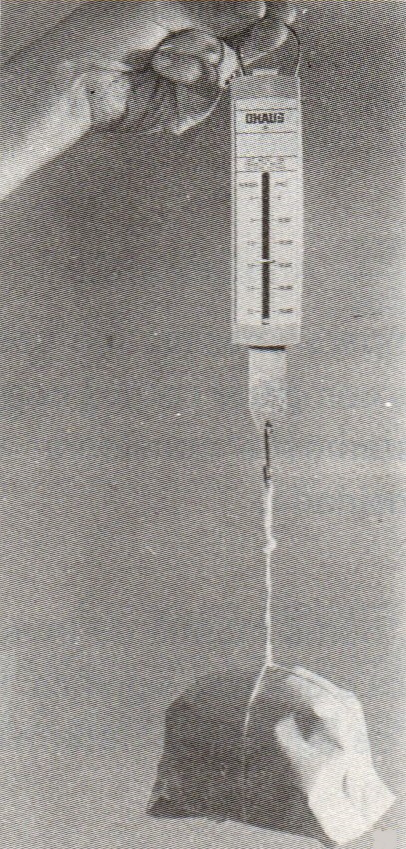
\includegraphics[height=7cm]{./image/PESTA/general/Balanca_Mola_1.jpg}
		\caption{Balança de Mola}
		\label{Balanca_Mola_1}
	\end{figure}
\end{minipage}
\newline
\newline
\newline
A balança por mola, como o nome implica, mede a pressão (ou sua tensão) exercido sobre a mola para determinar a massa do objeto. Este tipo de balanças ainda são muito comum nos dias de hoje por serem bastante económicas de fabricar, mas não tem tanta precisão como as eletrónicas desenvolvidas e aperfeiçoadas durante o século \textit{XX}.
\\
\\
As balanças eletrónicas mais modernas utilizam resistências elétricas em materiais permeáveis e fazer passar uma corrente elétrica na qual é possível detetar a variação de condutividade das resistências em que é proporcional a pressão exercida sobre esse material, podendo dai se deduzir o peso dos objetos que se encontrem na balança.
\\
\\
\\
\section{section}
\subsection{subsection}
\subsection{subsection}
\section{subsection}

	\newpage
	%%%%%%%%%%%%%%%%%%%%%%%%%%%%%%%%%%%%%%%%%%%%%%%%%%%%%%%%%%%%%%%%
\chapter{Balança Digital}
Para o desenvolvimento deste projeto, foi criado um kit de desenvolvimento para facilitar sua implementação, testar, efetuar alterações e melhoramentos.
\\
\\
Abaixo pode-se ver a montagem em esqueleto do equipamento utilizado na \textit{figura} \ref{Kit_Desenvolvimento_2},
\begin{figure}[H]
	\centering
	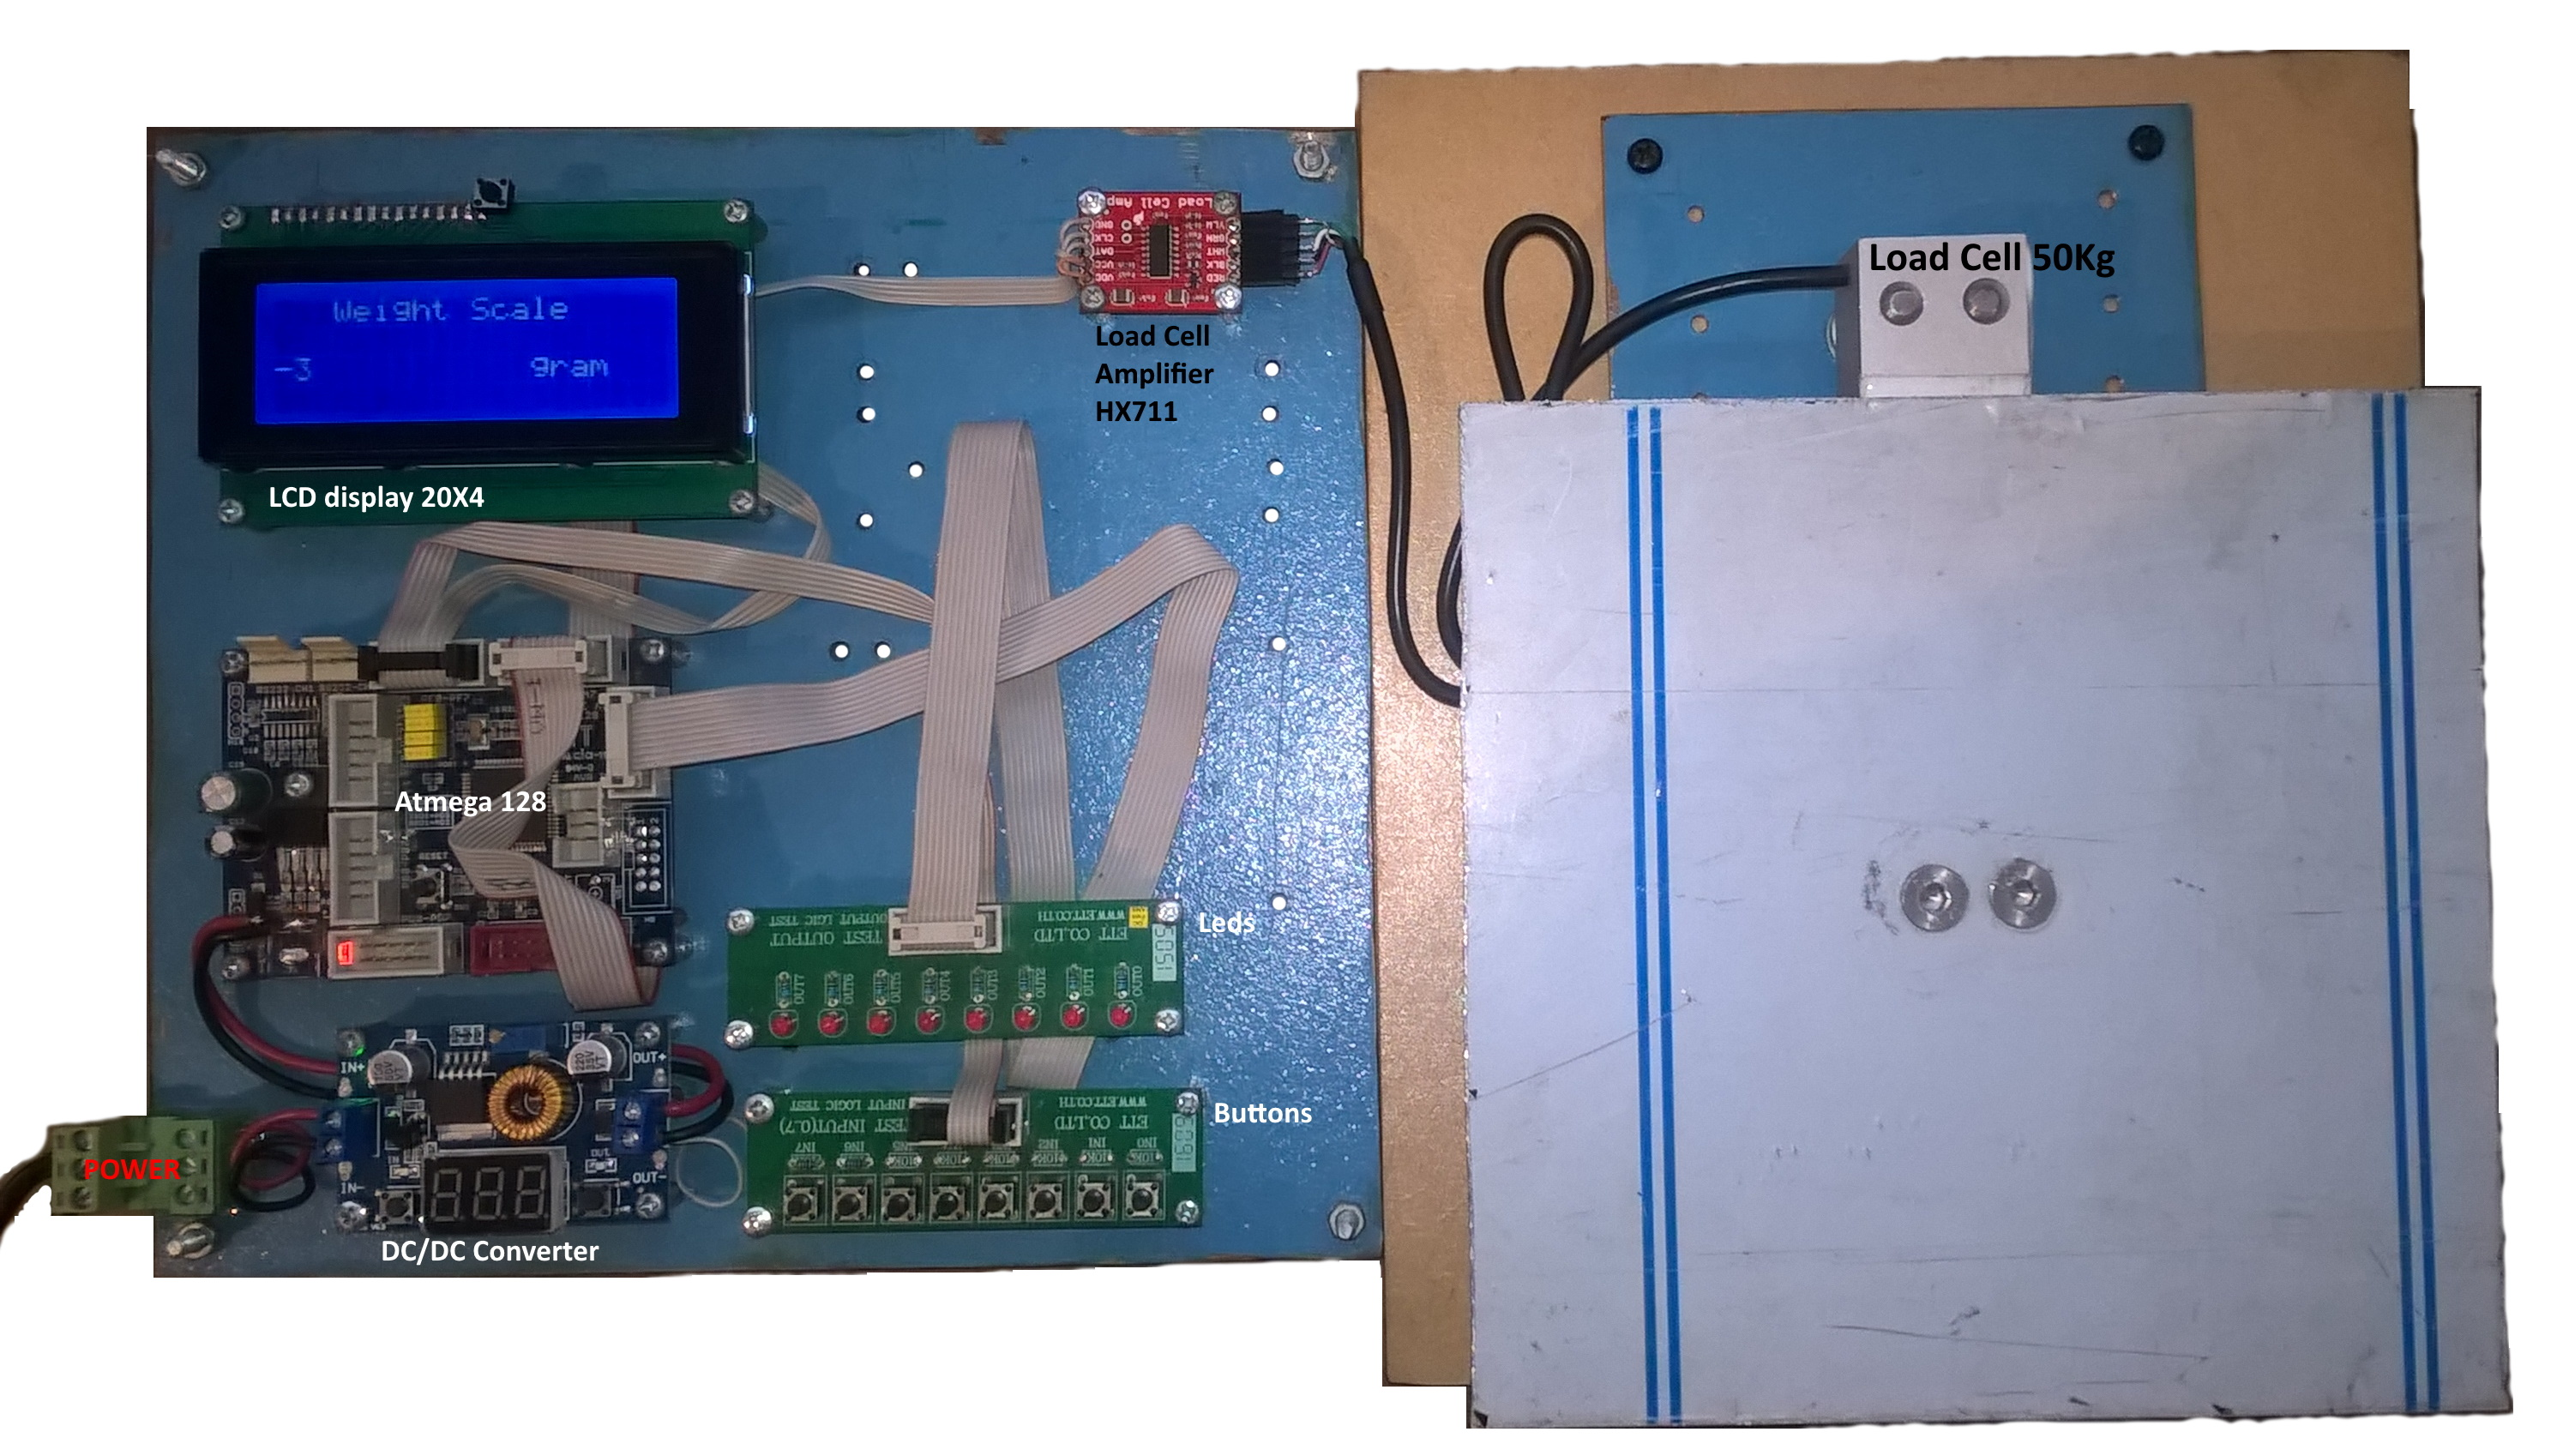
\includegraphics[scale=0.12]{./image/PESTA/kit/Kit_Desenvolvimento_2.jpg}
	\caption{Kit de Desenvolvimento}
	\label{Kit_Desenvolvimento_2}
\end{figure}
a seguir a \textit{figura} \ref{Block_diagram_1} representado os elementos em diagrama de blocos.
\begin{figure}[H]
	\centering
	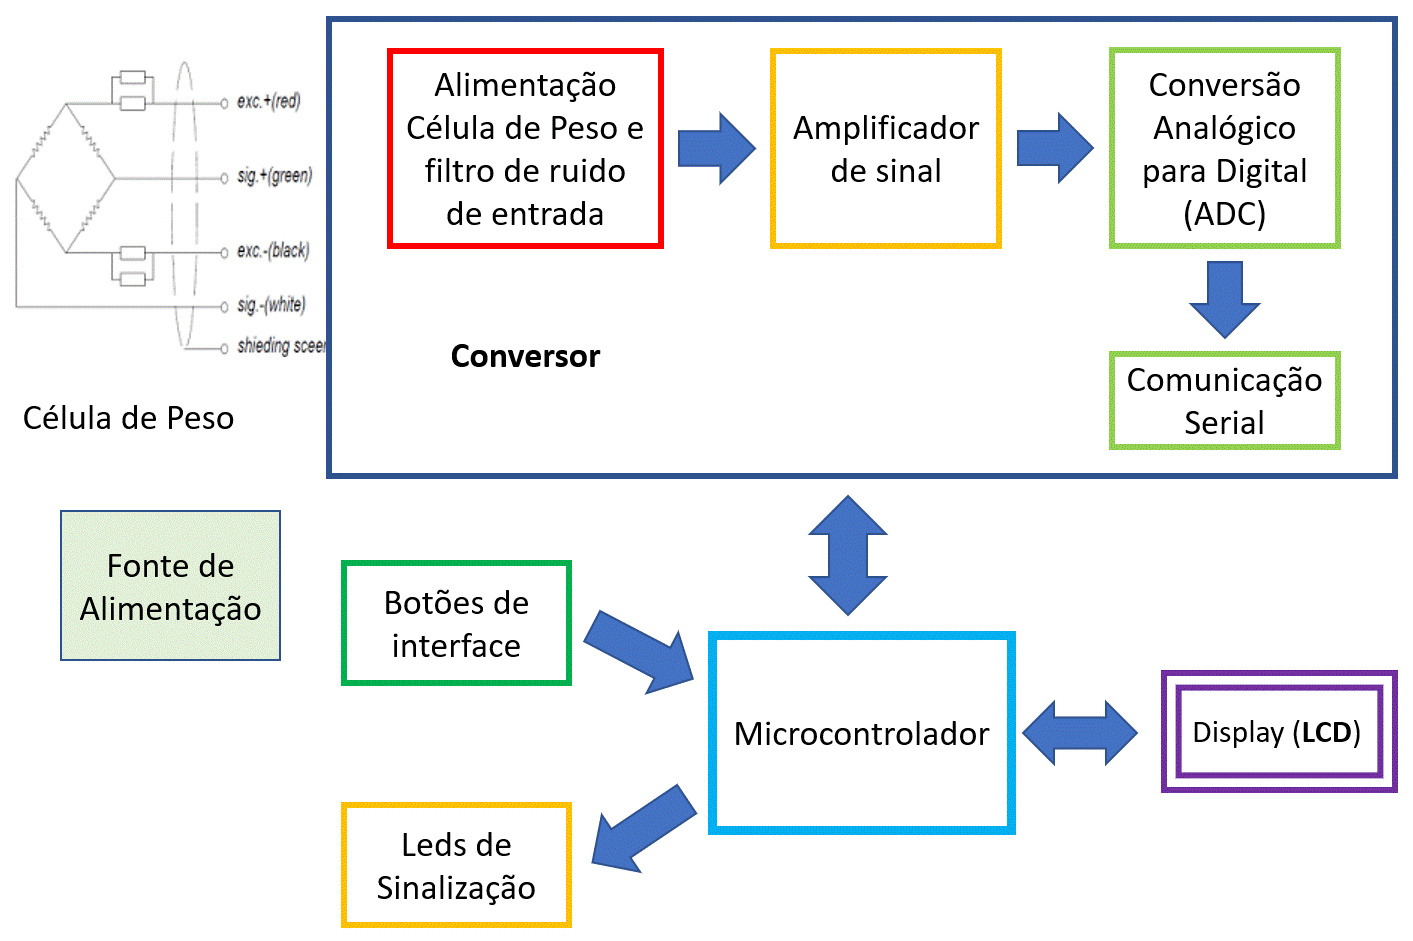
\includegraphics[scale=0.27]{./image/PESTA/Diagrama/Diagrama_bloco_3.jpg}
	\caption{Diagrama Blocos}
	\label{Block_diagram_1}
\end{figure}
\section{sensor}
Para medir a massa recorreu-se a uma \textbf{célula de peso} que determina a pressão exercida por um dado objeto, neste caso é um bloco de alumínio como indicado na \textit{figura} \ref{Load_Cell_1}, para isso ser possível este utiliza sensores Piezoresistivos numa montagem em ponte \textit{wheatstone} sobre essa superfície em locais determinados.
\\
\begin{figure}[H]
	\captionsetup{justification=raggedright,singlelinecheck=false}
	\flushleft
	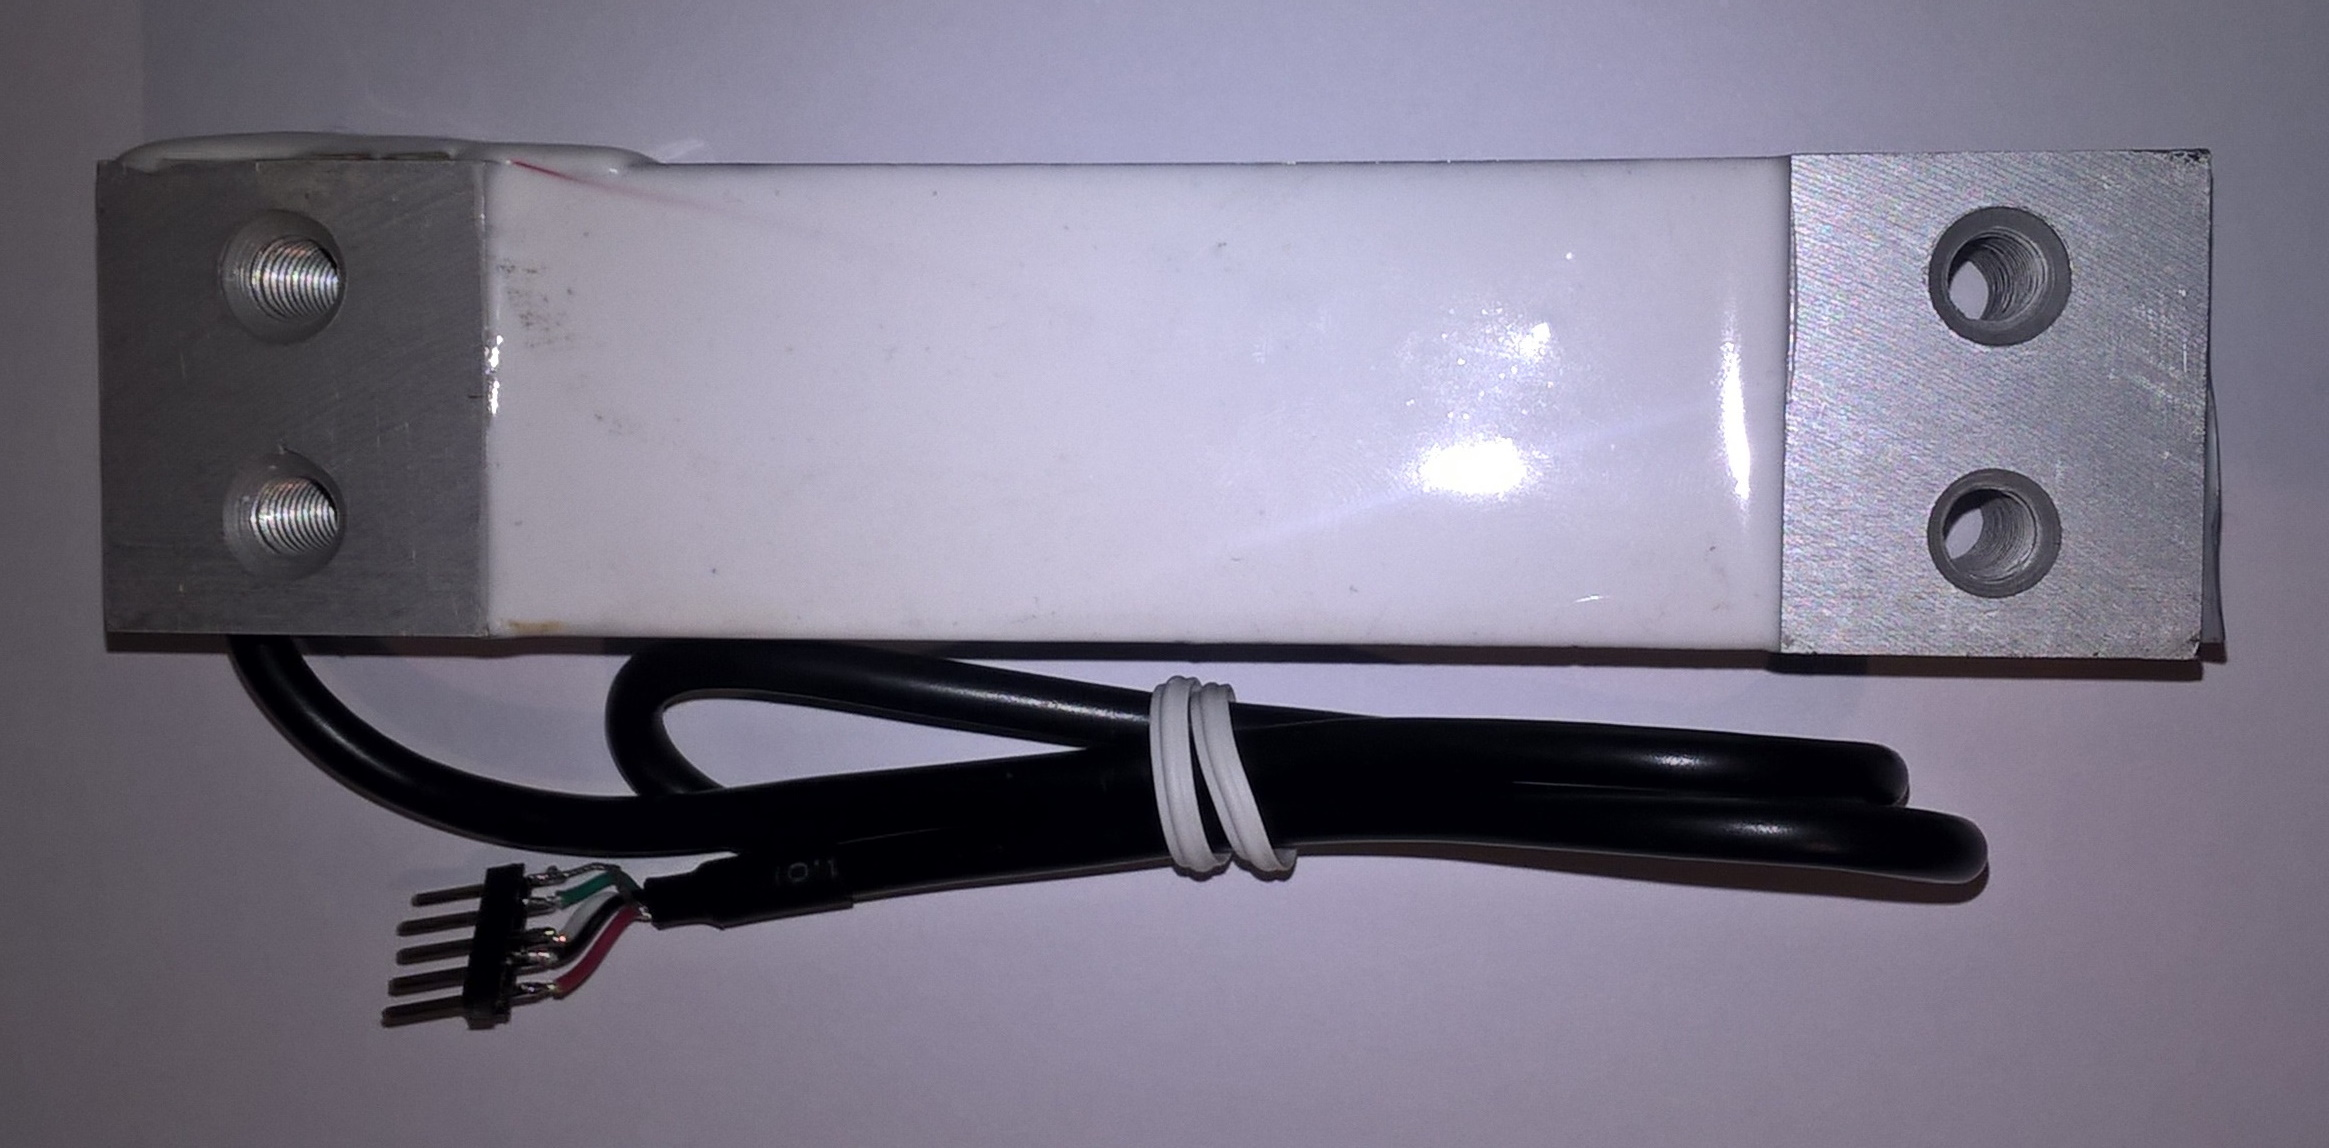
\includegraphics[scale=0.15]{./image/PESTA/material/Load_Cell_1.jpg}
	\caption{Célula de Peso 50Kg}
	\label{Load_Cell_1}
\end{figure}
\figurespace{.5}
Piezoresistividade deriva seu nome da palavra grega \textit{piezin}, que significa "pressionar". É um efeito exibido por vários materiais que exibem uma mudança na resistividade devido a uma pressão aplicada. O efeito foi descoberto pela primeira vez por Lord Kelvin em \textcolor{blue}{1856}, que notou que a resistência dos fios de cobre e ferro aumentava quando em tensão. Ele também observou que os fios de ferro apresentavam uma alteração maior na resistência do que os de cobre. A primeira aplicação do efeito piezoresistivo não apareceu até a década de \textcolor{blue}{1930}, cerca de \textcolor{blue}{75} anos após a descoberta de Lord Kelvin. Em vez de usar fios de metal, esses assim chamados medidores de tensão são geralmente feitos de uma folha de metal fina montada em uma película de suporte, que pode ser colada em uma superfície. O sensor de fita de metal típico é representado na \textit{figura} \ref{strain_gauge_1} \cite{book-9}.
\\
\\
\begin{minipage}[!b]{.5\linewidth}
\begin{figure}[H]
	\captionsetup{justification=raggedright,singlelinecheck=false}
	\flushleft
	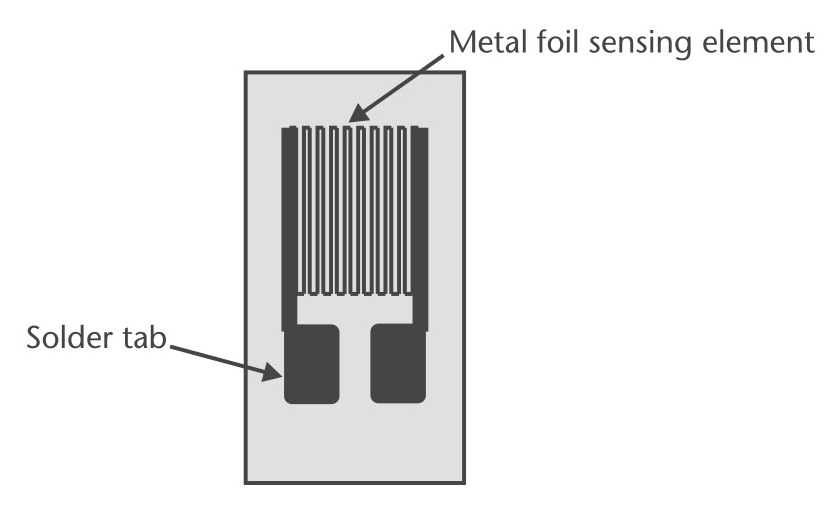
\includegraphics[height=5cm]{./image/PESTA/general/strain_gauge_1.jpg}
	\caption{Fita metálica \textit{strain gauge} \cite{book-9}}
	\label{strain_gauge_1}
\end{figure}
\end{minipage}
\begin{minipage}[!b]{.5\linewidth}
\begin{figure}[H]
	\captionsetup{justification=raggedright,singlelinecheck=false}
	\flushleft
	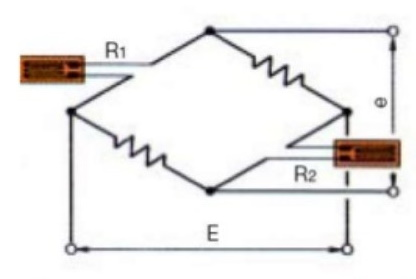
\includegraphics[height=5cm]{./image/PESTA/schematic/Wheatstone_2.jpg}
	\qquad \caption{Ponte \textit{Wheatstone}}
	\label{wheatstone_2}
\end{figure}
\end{minipage}
\minipagespace{.5}
\begin{minipage}[!b]{.4\linewidth}
	\begin{figure}[H]
		\captionsetup{justification=raggedright,singlelinecheck=false}
		\flushleft
		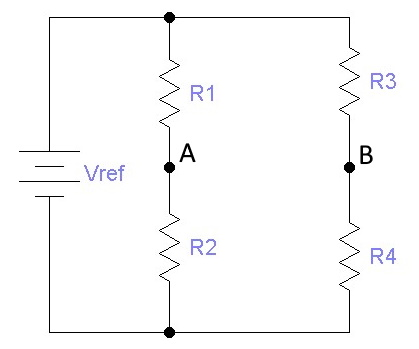
\includegraphics[height=5cm]{./image/PESTA/schematic/Wheatstone_1.jpg}
		\caption{\textit{Wheatstone} por resistências}
		\label{wheatstone_1}
	\end{figure}
\end{minipage}
\begin{minipage}[!b]{.6\linewidth}
	\begin{align}
		\label{eq:wheatstone}
		&V_A =  \frac{R_2}{R_1 + R_2} \; V_{ref} \; V_B=\frac{R_4}{R_3 + R_4} \; V_{ref} \\
		&V_{AB} =  V_A - V_B = e \\
		&V_{AB}= \left(\frac{R_2}{R_1 + R_2} - \frac{R_4}{R_3 + R_4}\right) \; Vref \\
		&e = \frac{R_2 R_3 - R_4 R_1}{(R_1 + R_2)(R_3 + R_4)} \; Vref
	\end{align}
	\minipagespace{.1}
\end{minipage}
\minipagespace{.5}
Normalmente nestas aplicações só é usados um sensor ou dois sensores em que estão nos extremos opostos  ou ligados ao mesmo ponto da alimentação, só em casos muito raros são utilizados os quatro sensores na qual a sensibilidade é máxima. E como é óbvio se o valor das quatro resistências são iguais $V_{AB}$ na saída é nula, e quando se utiliza apenas dois sensores a sensibilidade do sistema é intermédia.
\newpage
A montagem da mesa de medição \textit{figura} \ref{Prato},
\minipagespace{5}
\begin{minipage}[!b]{\linewidth}
\begin{figure}[H]
	\centering
	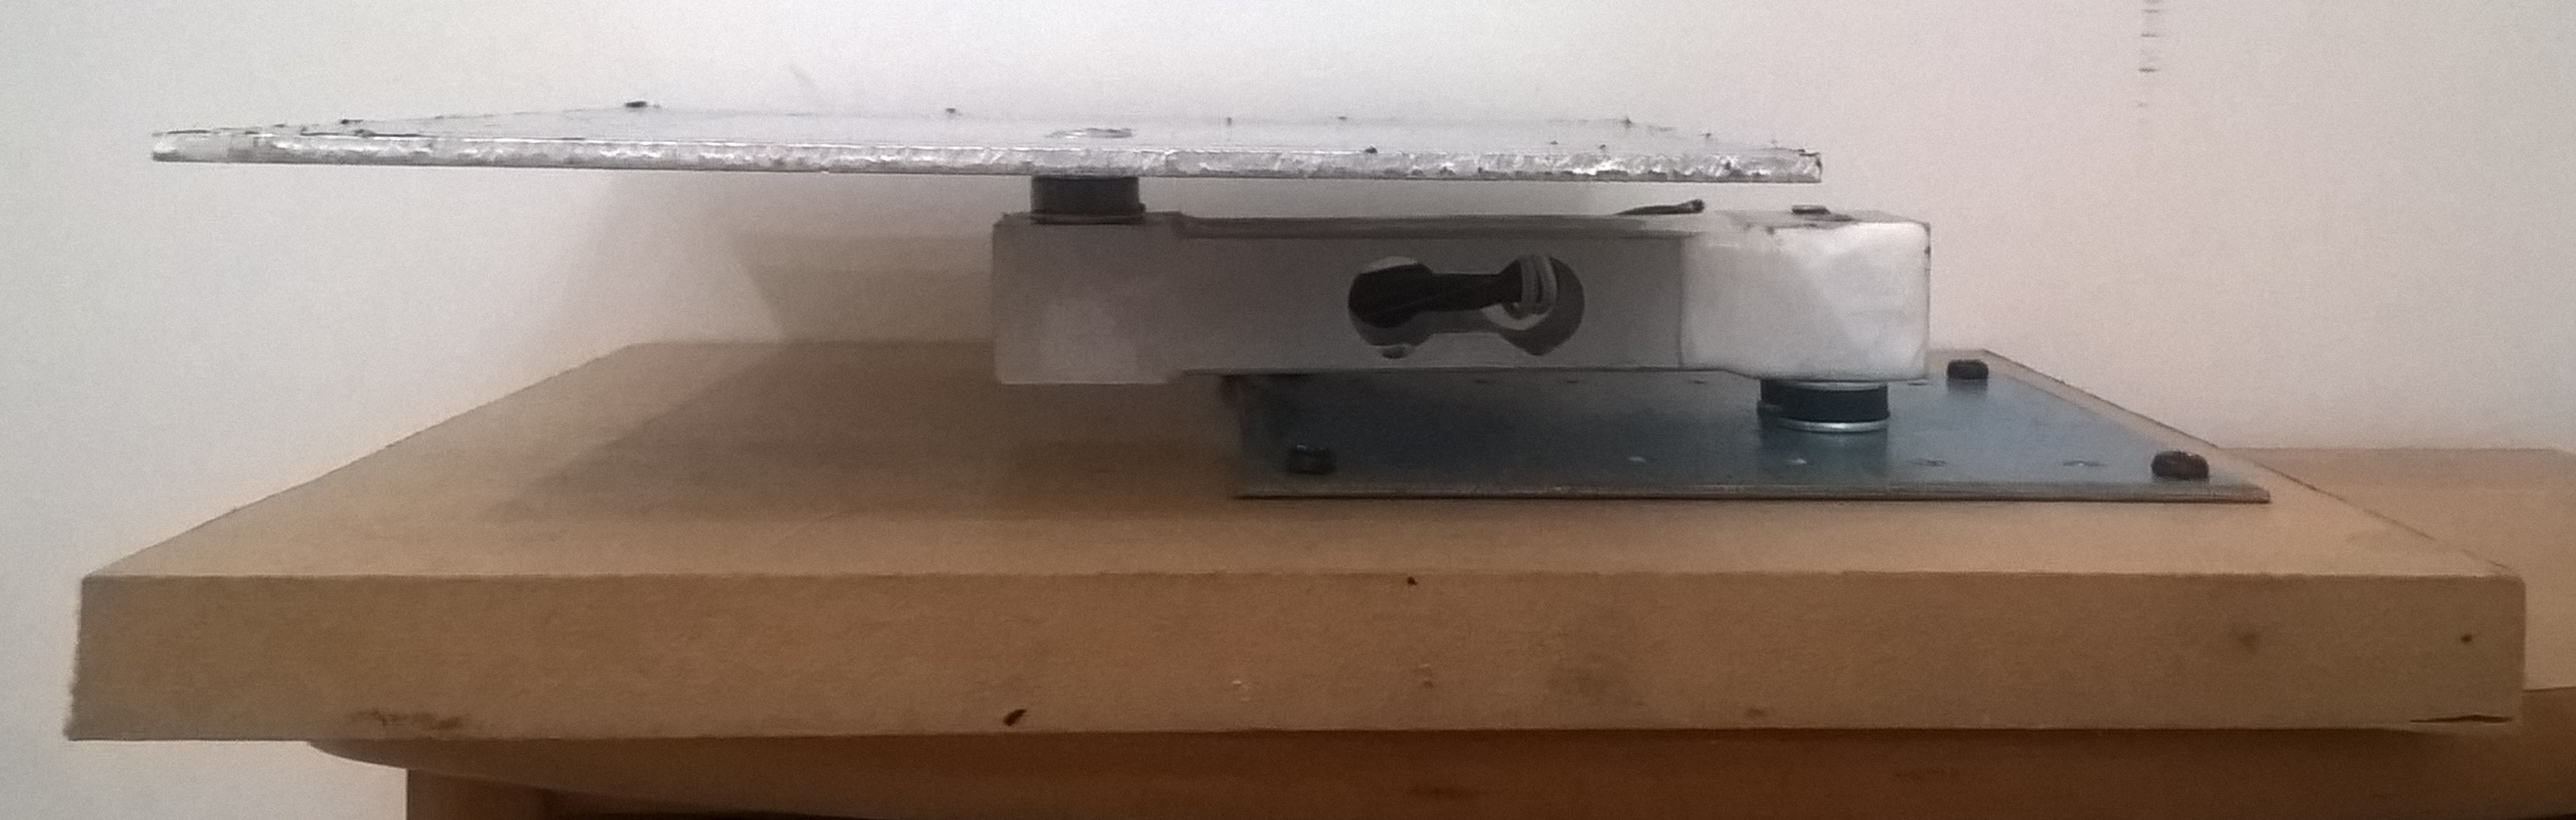
\includegraphics[scale=0.16]{./image/PESTA/material/Prato.jpg}
	\caption{Prato}
	\label{Prato}
\end{figure}
\end{minipage}
\newpage
\section{Amplificador de sinal}
A amplificação é geralmente um requisito fundamental, pois a maioria dos sensores tende a produzir níveis de sinal significativamente mais baixos do que aqueles usados no processador digital. Sensores resistivos podem precisar de um amplificador de carga. Se possível, é vantajoso ter o ganho o mais próximo possível do elemento sensor. Em situações onde um alto ganho é necessário, muitas vezes pode haver implicações para lidar 
com quaisquer efeitos adversos, como o ruído, também em termos de \textit{layout} do \textit{chip}, os transitórios agudos associados aos sinais digitais precisam ser mantidos bem longe dos circuitos analógicos \textit{front-end}. \cite{book-9}
\\
\\
A ligação destes componentes é intuitivo e fácil de se perceber, o que é complexo neste trabalho é a interligação destes equipamentos com o micro-controlador por meio de \textit{software} e criar o \textit{driver} de comunicação para a placa do amplificador de sinal, já que o protocolo de comunicação é proprietário.
\\
\\
\begin{figure}[H]
	\captionsetup{justification=raggedright,singlelinecheck=false}
	\centering
	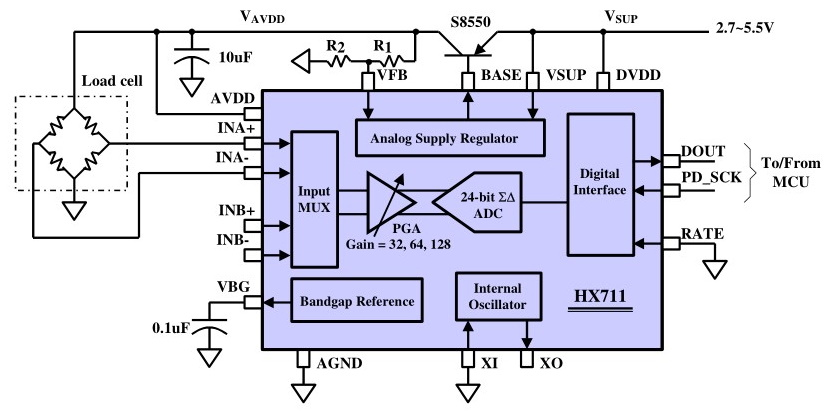
\includegraphics[scale=0.35]{./image/PESTA/schematic/HX711_Schematic_1.jpg}
	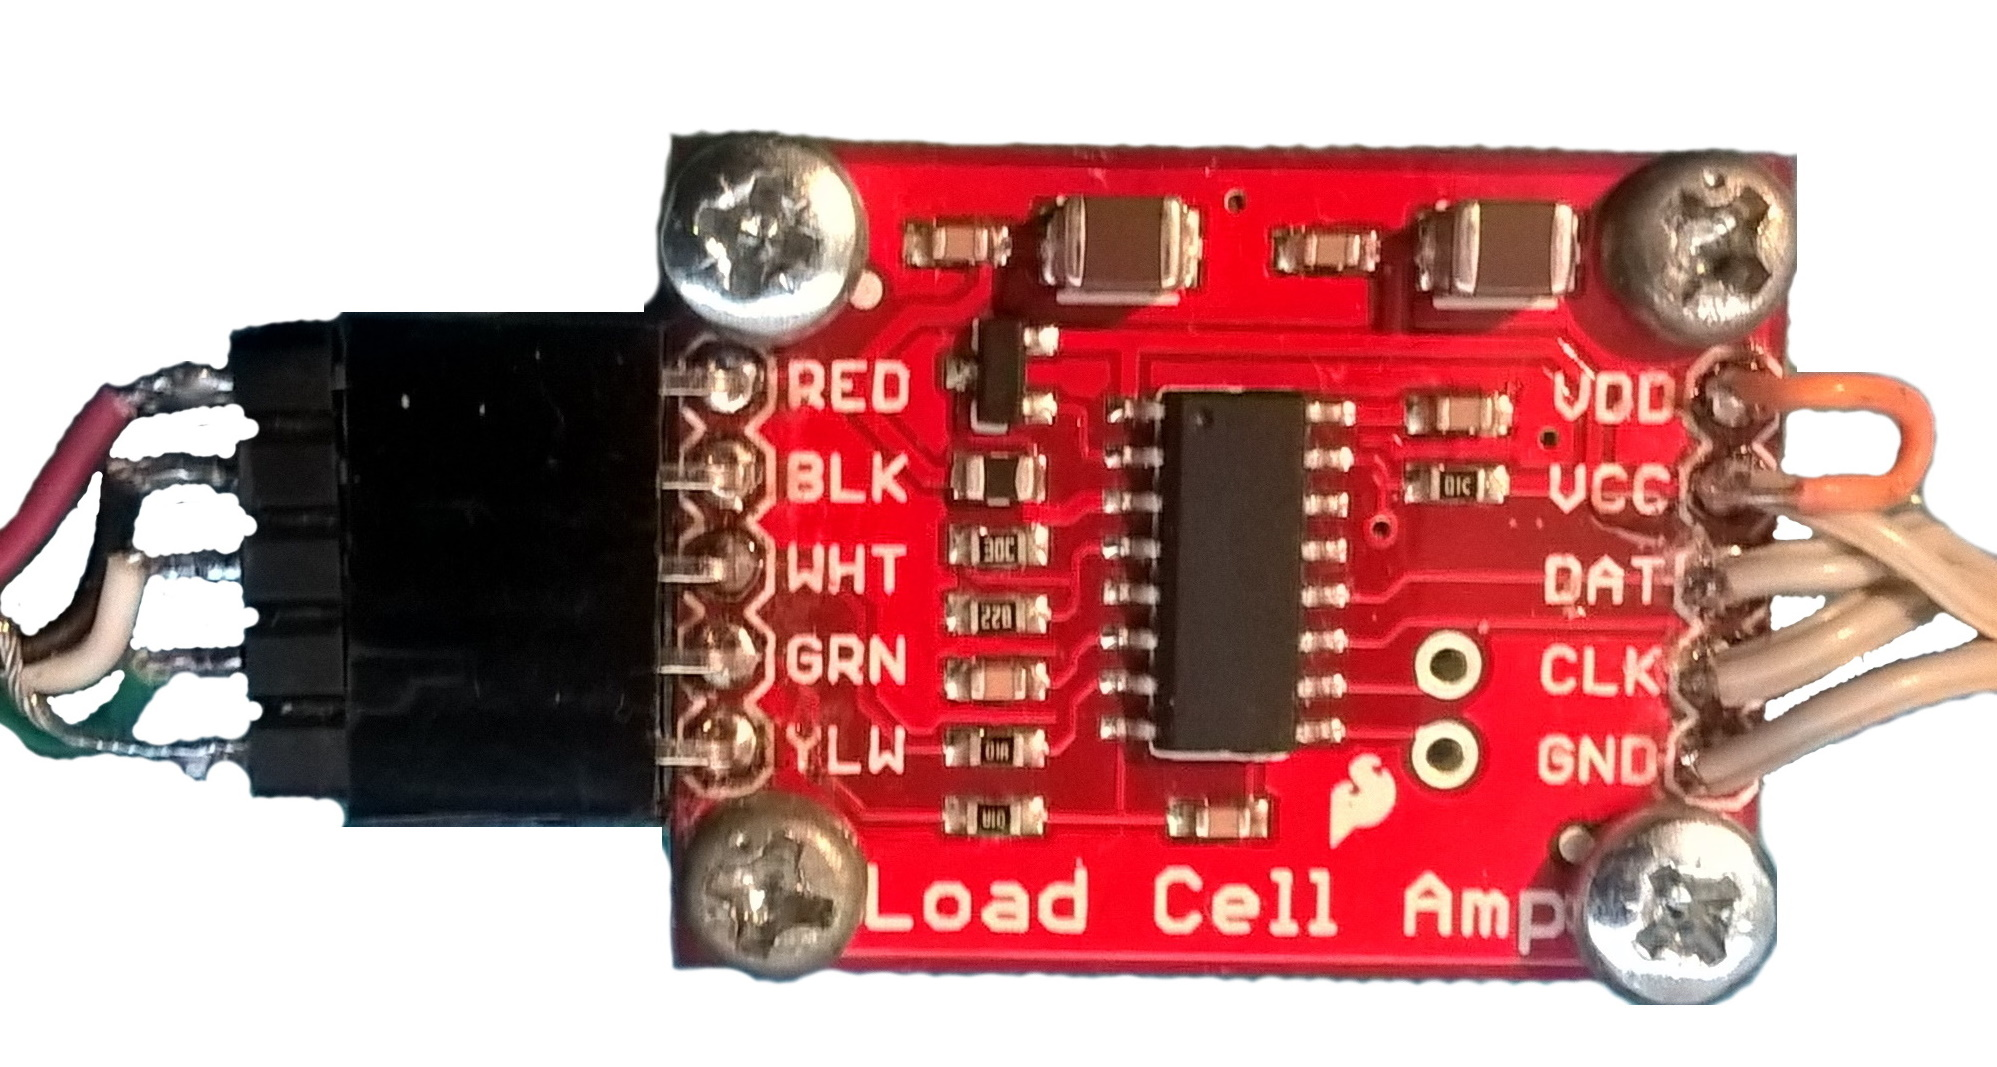
\includegraphics[scale=0.1]{./image/PESTA/material/HX711_board_1.jpg}
	\caption{Amplificador de Sinal [HX711]}
	\label{HX711_Schematic_1}
\end{figure}
\figurespace{.5}
A placa \textit{Load Cell Amplifier }pode ser programada fisicamente para determinar o numero de amostras por segundo a ser transmitido, tem opção de \textcolor{blue}{10} amostras por segundo e \textcolor{blue}{80} amostras, neste projeto optei pela segunda opção que necessita alteração na placa de circuito de impresso, isto é, abrir o \textit{jumper} respetivo de configuração.
\\
\\
\begin{table}[H]
	\centering
	\caption{Terminais HX711 ({\tiny \scriptsize{top view}})}
	\begin{tabular}{||L{1cm} C{3cm} | p{3cm}  C{2cm}||}
		\hline
		\multicolumn{2}{||c|}{MCU} & \multicolumn{2}{|c||}{\textit{Célula de peso}}\\ [1ex]
		\hline
		1 & GND & EARTH (GND) & YLW \\ 
		2 & CLK & INPA & GRN \\
		3 & DATA & INNA & WHT \\
		4 & VCC &  GND & BLK \\
		5 & VDD & $V_{ADC}$ & RED \\ [1ex]
		\hline
	\end{tabular}	
	\label{HX711_connection}
\end{table}
\tablespace{.5}
A conversão de informação é a transição entre o sinal continuo da vida real para um sinal discreto associado ao mundo digital, tipicamente esta etapa consiste na conversão analógica para digital.
\\
O processamento digital pode consistir de rotinas para compensar os desvios por linearização, compensação da sensibilidade e \textit{offset}, ou podem ser técnicas mais sofisticadas como reconhecimento de padrões (tais como redes neuronais) para equipamentos de sensores vetoriais.\cite{book-9}
\\
A comunicação trata de cuidar das rotinas necessárias para transferir e receber a informação e sinais de controle para a linha de comunicação com o sensor, e o processador que toma lugar como componente central tratando a informação, guardar os dados e fazer rotinas tais como de calibração, teste e controlo de ganho da amplificação. \cite{book-9}
\\
\\
\begin{figure}[H]
	\centering
	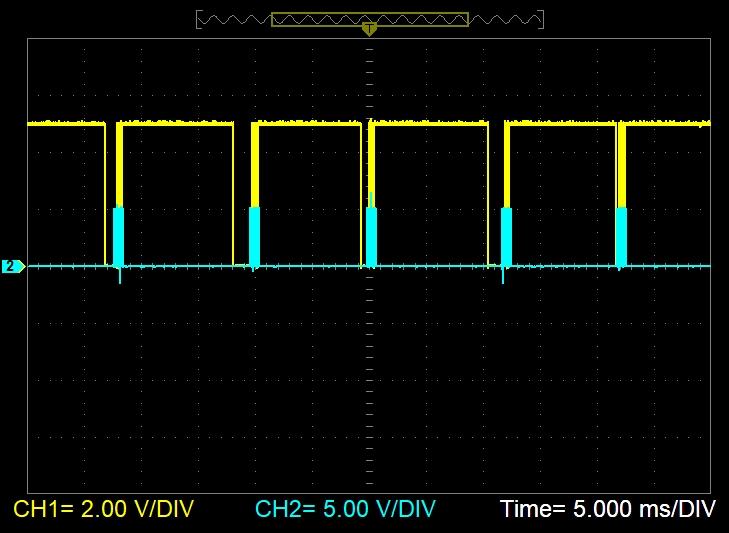
\includegraphics[scale=0.55]{./image/PESTA/graph/80SPS64GAIN/SPS_80.JPG}
	\caption{Amostras}
	\label{SPS_64}
\end{figure}
\figurespace{.5}
A livraria (\textit{driver}) criada recorre a interrupções periódicas quando o sinal de \textit{data} vai para a massa, indicando assim que tem um pacote de leitura pronto a ser transmitido.
\\
\\
\begin{minipage}[!b]{.40\linewidth}
	\begin{table}[H]
		\captionsetup{justification=raggedright,singlelinecheck=false}
		\caption{Configuração Ganho}
		\begin{tabular}{ | c | c | c |  }
			\hline
			\makecell[c]{PD\_SCK \\ Impulsos} & Entrada  & Ganho \\
			\hline
			\hline
			25 & \textbf{A} & 128 \\
			\hline
			26 & \textbf{B} & 32 \\
			\hline
			27 & \textbf{A} & 64 \\
			\hline
		\end{tabular}
		\label{Gain_Selection}
	\end{table}
	\tablespace{2}
\end{minipage}
\begin{minipage}[l]{.6\linewidth}
\vspace{.3cm}
Como indicado abaixo no gráfico em que a linha \textcolor{yellow}{amarela} é a informação e a linha \textcolor{BlueGreen}{azul} o respetivo \textit{clock} que é gerado pelas interrupções do micro-controlador fazendo \textit{shift} dos \textcolor{blue}{24} bits, que depois no fim transmite para o amplificador o ganho de amplificação a ser usado pelo numero excedente de \textit{clock cycles}, em que nesta demonstração \textit{figura} \ref{Gain_128_example} é \textcolor{blue}{um}, e corresponde a ganho de \textcolor{blue}{128}, respeitando a \textit{tabela} \ref{Gain_Selection},  e a sequir o exemplo da \textit{figura} \ref{Gain_64_example} com o ganho de \textcolor{blue}{64}, pois tem \textcolor{blue}{três} impulsos excedentes.
\\
\end{minipage}
\minipagespace{.5}
\begin{minipage}[!b]{.5\linewidth}
\begin{figure}[H]
	\captionsetup{justification=raggedright,singlelinecheck=false}
	\flushleft
	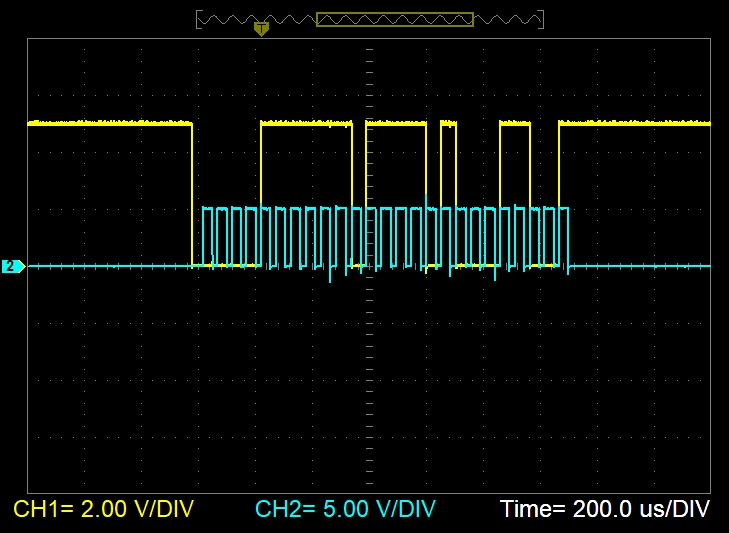
\includegraphics[scale=0.25]{./image/PESTA/graph/80SPS128GAIN/Gain_128_example.JPG}
	\caption{Ganho de 128}
	\label{Gain_128_example}
\end{figure}
\end{minipage}
\hspace{1cm}
\begin{minipage}[!b]{.5\linewidth}
\begin{figure}[H]
	\captionsetup{justification=raggedright,singlelinecheck=false}
	\flushleft
	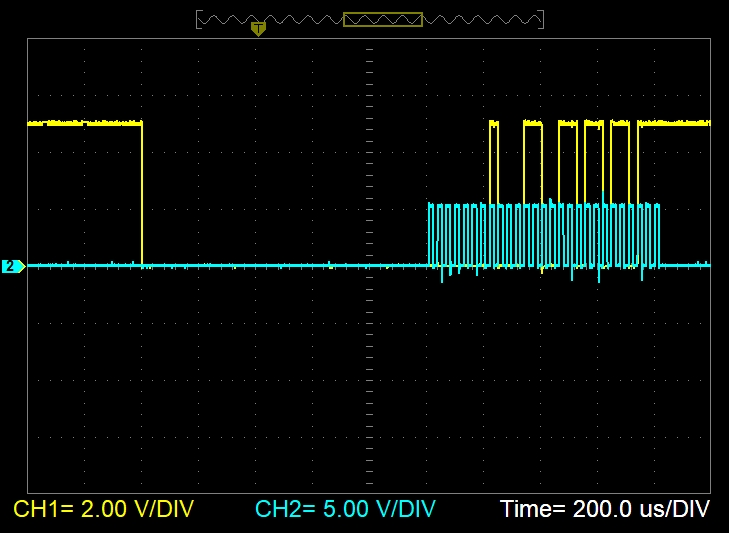
\includegraphics[scale=0.25]{./image/PESTA/graph/80SPS64GAIN/Gain_64_example.JPG}
	\caption{Ganho de 64}
	\label{Gain_64_example}
\end{figure}
\end{minipage}
\minipagespace{.5}
Para obter este resultado a livraria driver para o \textit{Load Cell Amplifier} teve de ter em consideração que o microcontrolador é de \textcolor{blue}{8} bits, porque o pacote de informação consiste de \textcolor{blue}{24} \textit{bits} e em que é transmitido primeiro o \textit{bit} \textbf{MSB}.
\\
\\
O código que executa esta rotina é demonstrado na \textit{figura} \ref{read_raw} que é chamada pelas interrupções periódicas e só é ativa quando a função na \textit{figura} \ref{Main_While_Balanca} \textbf{hx.query(\&hx)} é verdadeira.
\\
\\
\begin{minipage}[l]{\linewidth}
\begin{minipage}[l]{.60\linewidth}
\begin{figure}[H]
	\flushleft
	\captionsetup{justification=raggedright,singlelinecheck=false}
	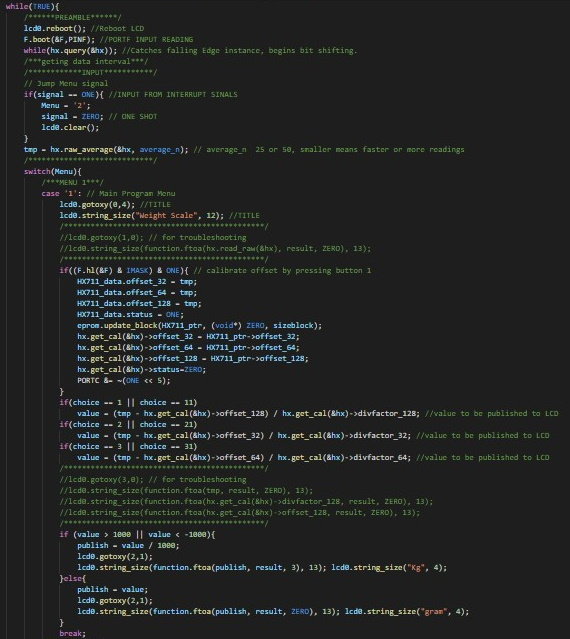
\includegraphics[scale=0.55]{./image/PESTA/Code/Main_While_Balanca.jpg}
	\caption{PROGRAM 1}
	\label{Main_While_Balanca}
\end{figure}
\end{minipage}
\begin{minipage}[l]{.33\linewidth}
	\vspace{1.1cm}
	\begin{figure}[H]
		\flushleft
		\captionsetup{justification=raggedright,singlelinecheck=false}
		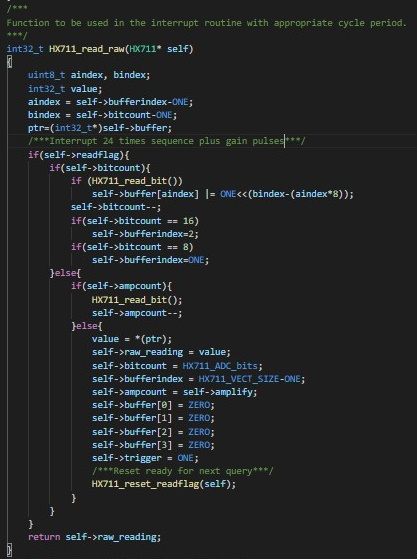
\includegraphics[scale=0.55]{./image/PESTA/Code/read_raw.jpg}
		\caption{Leitura ADC}
		\label{read_raw}
	\end{figure}
\end{minipage}
\end{minipage}
\minipagespace{.5}
Após obter um numero determinado de valores discretos é calculado sua média
\begin{equation}
	\label{eq:Mean}
	\overline{x}  =  \frac{1}{n}\sum_{i=1}^n x_i
\end{equation}
para ser tratado e deduzido o valor correspondente da massa.
\newpage
\section{Display LCD}
O \textit{Liquid-Crystal Dispaly} (\textbf{LCD}) utilizado é de 4x20, isto é, quatro linhas de vinte caracteres cada, é o interface humano principal, e durante o projecto uma ferramenta extremamente útil também para fazer \textit{debug} e executar testes no código.
\\
\\
Uma livraria na qual já tinha feito para outros projetos serviu para aplicar neste, poupando bastante tempo, revelando a importância de documentar os conhecimentos adquiridos. A livraria ou se preferem \textit{driver} esta \textit{anexado}.
%[\ref{codigo}]
\\
\\
Abaixo esta uma tabela \ref{LCD_connections} com as respetivas ligações.
\tablespace{.2}
\begin{table}[H]
	\centering
	\caption{Conexões \textbf{LCD}}
	\begin{tabular}{||p{1cm} p{2cm} p{4cm} | p{1cm}||} 
		\hline
		\multicolumn{3}{||c|}{\textbf{LCD Pin}} & \multicolumn{1}{|c||}{\textbf{MCU Pin}}\\ [1ex]
		\hline
		1 & VSS & GND & \\
		2 & VCC & +5V & \\
		3 & VEE & \textit{Contrast Control} & \\
		4 & RS & \textit{Register Select} & Pin 0 \\
		5 & RW & \textit{Read/Write} & Pin 1 \\
		6 & E & \textit{Enable} & Pin 2 \\
		7 & Do & \textit{Data Pin 0} & \\
		8 & D1 & \textit{Data Pin 1} & \\
		9 & D2 & \textit{Data Pin 2} & \\
		10 & D3 & \textit{Data Pin 3} & \\
		11 & D4 & \textit{Data Pin 4} & Pin 4 \\
		12 & D5 & \textit{Data Pin 5} & Pin 5 \\
		13 & D6 & \textit{Data Pin 6} & Pin 6 \\
		14 & D7 & \textit{Data Pin 7} & Pin 7 \\
		15 & LED+ & \textit{Led +5V} &  \\
		16 & LED- & \textit{Led Ground} & \\
		\multicolumn{3}{||c|}{\textit{Reboot} LCD} & \multicolumn{1}{|l||}{Pin 3}\\ [1ex]
		\hline
	\end{tabular}	
	\label{LCD_connections}
\end{table}
\begin{figure}[H]
	\centering
	%%\captionsetup{justification=raggedright,singlelinecheck=false}
	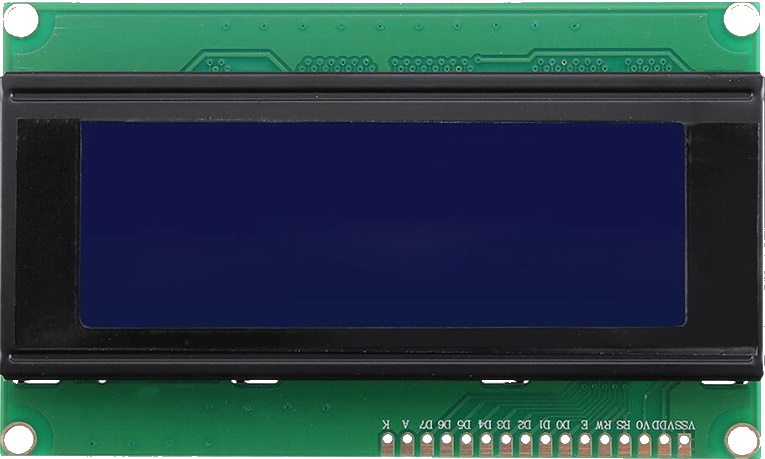
\includegraphics[scale=.5]{./image/PESTA/material/4x20_LCD.jpg}
	\caption{LCD}
	\label{4x20_LCD}
\end{figure}
\newpage
\section{Micro-controlador}
Os microcontroldores da \textbf{Atmel} de 8 e 32 bits são baseados na arquitetura avançada de \textbf{Harvard} na qual esta concebido para baixos consumos e performance.
\\
\\
Este tipo de arquitetura tem dois  \textit{busses} (barramentos) um dedicado a leitura das instruções a executar e outra para escrita e leitura de \textit{data} (informação ou dados), isto assegura que uma nova instrução pode ser executada em cada ciclo de relógio, na qual elimina estados de espera quando não ha instruções prontas a executar.
\\
\\
Nos microcontroladores da \textbf{AVR} os barramentos estão configurados de forma a dar prioridade ao barramento das instruções do \textbf{CPU} acesso a memoria flash enquanto o barramento da CPU de dados tem prioridade de acesso a \textbf{SRAM} (Static Random Access Memory).
\\
\\
O espaço de memoria de dados é dividida em três, os \textbf{GPR} (General Purpose Registers) as \textbf{SFRs} (Special Function Registers) ou memoria de I/O e a \textit{data} \textbf{SRAM}.
\\
\\
Os microcontroladores da \textbf{AVR} utiliza uma arquitetura de instruçõeses \textbf{RISC} (Reduced Instruction Set Computer ou Reduced COMPLEXITY Instruction Set Computer) na qual reduz a complexidade dos circuitos na codificação de cada instrução.
\\
\\
Dai que os microcontroladores que se baseiam nestes tipos de arquitetura são sinonimo de código reduzido, alta performance e baixo consumo energético.
\\
\\
\begin{figure}[H]
	\centering
	%%\captionsetup{justification=raggedright,singlelinecheck=false}
	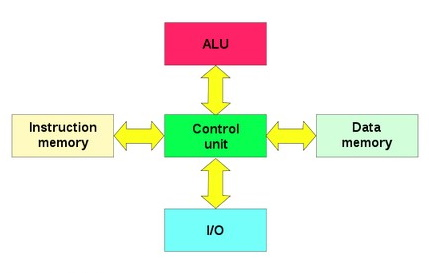
\includegraphics[scale=1]{./image/PESTA/Diagrama/Harvard_architecture.jpg}
	\caption{Harvard Architecture}
	\label{Harvard_architecture}
\end{figure}
\qquad link: \url{https://en.wikipedia.org/wiki/Harvard_architecture}
\newpage
Neste projeto apostei no Atmega 128 (\textit{figura} \ref{Atmega_128_pinagem}) por ser um dos mais poderosos \textbf{MCU´s} da linha de 8 b\textit{bit} da Atmel, também por estar integrado já numa placa de desenvolvimento usando o sistema por fichas \textit{insulation-displacement contact} (\textbf{IDC}) que prefiro, ou seja, usando \textit{flatcables} para ligar os periféricos, e considero muito mais pratico do que sistema que esta na moda, tais como a linha Arduino e da STM por ter um interface por pinos.
\\
\\
\\
\\
\\
\begin{figure}[H]
	\centering
	%%\captionsetup{justification=raggedright,singlelinecheck=false}
	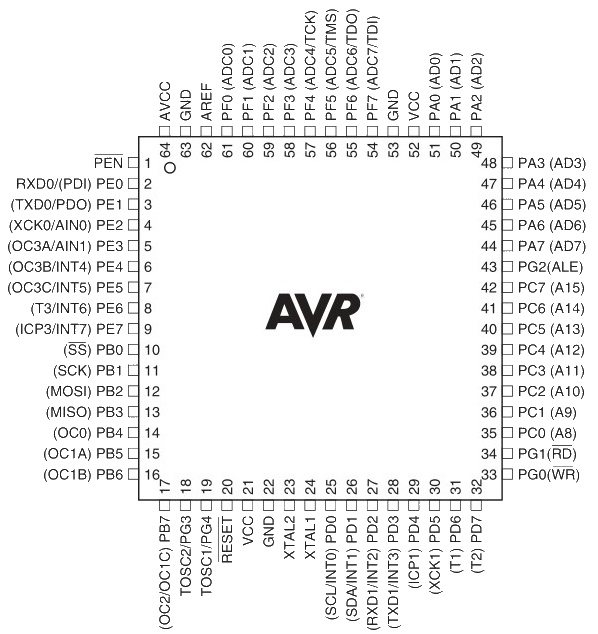
\includegraphics[scale=0.7]{./image/PESTA/material/Atmega128_1.jpg}
	\caption{Atmega 128}
	\label{Atmega_128_pinagem}
\end{figure}
\figurespace{1}
{Transparências Sistemas Digitais 2 \quad \textbf{ISEP} \quad 2008/2009 \quad \textit{link}}:
\\
\url{https://drive.google.com/file/d/1wgOGf8WwYY0OzDhRca9ypXz-iBO55YOF/view?usp=sharing}
\newpage
A características do micro-controlador ATmega 128 esta abaixo indicados na lista, os temporizadores considero o mais importante, o ADC nem vai ser usado neste projeto a alternativa é muito melhor, talvez os MCU nem deviam ter esta funcionalidade e realçar em meios de comunicação e memoria com as livrarias já disponíveis, este integrado é perfeito para esta aplicação em causa, sempre que fazemos projetos também temos de considerar os MCU de 32 \textit{bit} mas existe uma linha muito fina de apostar noutra alternativa e trabalhar com um sistema operativo devido a complexidade exigida, muito mais configurações e opções disponíveis do que um micro-controlador de 8 e 16 \textit{bit}.
\\
\\
\begin{minipage}{\linewidth}
{\Large Caracteristicas do Atmega 128 :}
\begin{itemize}	
	\setlength\itemsep{-0.7em}
	\item Arquitectura RISC
	\item 33 instruções (a maior parte executada num único ciclo de execução)
	\item 32 x 8 registos de trabalho (arquitectura de registos)
	\item Até 16 MIPS (@16MHz) – 62.5ns / instrução
	\item 64K x 16 palavras de programa – 128K bytes FLASH
	\item 4K bytes de RAM interna
	\item 4K bytes de E2PROM de dados
	\item Ciclos de escrita / leitura – FLASH=10000, E2PROM=100000
	\item 7 Portos de IO \\
		\hspace*{.5cm}	-> 6 x 8 bits (Portos A .. F) \\
		\hspace*{.5cm}	-> 1 x 5 bits (Porto G)
	\item 2 x Timer / Counter de 8 bits
	\item 2 x Timer / Counter de 16 bits
	\item 1 x Real Time Counter ( com oscilador independente)
	\item 2 x PWM de 8 bits
	\item 6 x PWM de 16 bits
	\item ADC de 10 bits (8 canais)
	\item 2 x USART
	\item SPI
	\item TWI (I2C)
\end{itemize}
\end{minipage}
\minipagespace{0.2}
Para programar este microcontrolador (\textbf{Atmega 128}) foi utilizado o programador da marca da Atmel precisamente o \textbf{Atmel-ICE} \textit{figura} \ref{Programador_1}, que para este equipamento tem disponível programação via \textit{In-System Programming} (\textbf{ISP}) \textit{figura} \ref{ISP_6_8_10pin} e \textit{Joint Test Action Group} (\textbf{JTAG}).
\minipagespace{.2}
\begin{minipage}[!b]{.5\linewidth}
	\begin{figure}[H]
		\captionsetup{justification=raggedright,singlelinecheck=false}
		\flushleft
		\includegraphics[scale=0.75]{./image/PESTA/programador/Atmel_ice.png}
		\caption{Diagrama Blocos}
		\label{Programador_1}
	\end{figure}
\end{minipage}
\hspace{.5cm}
\begin{minipage}[!b]{.5\linewidth}
	\begin{figure}[H]
		\captionsetup{justification=raggedright,singlelinecheck=false}
		\flushleft
		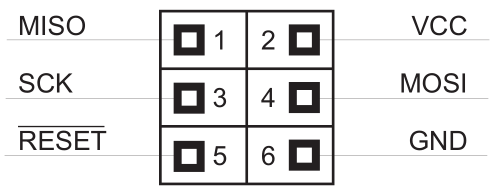
\includegraphics[scale=0.45]{./image/PESTA/programador/isp_6pin.png}
		\hspace{.3cm}
		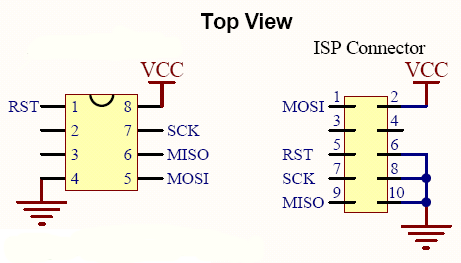
\includegraphics[scale=0.5]{./image/PESTA/programador/isp_8e10pin.png}
		\caption{Fichas \textbf{ISP}}
		\label{ISP_6_8_10pin}
	\end{figure}
\end{minipage}
\chapter{Software}
O \textbf{IDE} utilizado neste trabalho foi o \textbf{\textit{{Microchip Studio for AVR\textsuperscript{\textregistered} and SAM Devices}}} (\textit{version: 7.0.2542}). A programação foi feita em Linguagem \textbf{C}, sua estrutura sintática esta abaixo mencionado:
\\
\\
\begin{figure}[H]
	\centering
	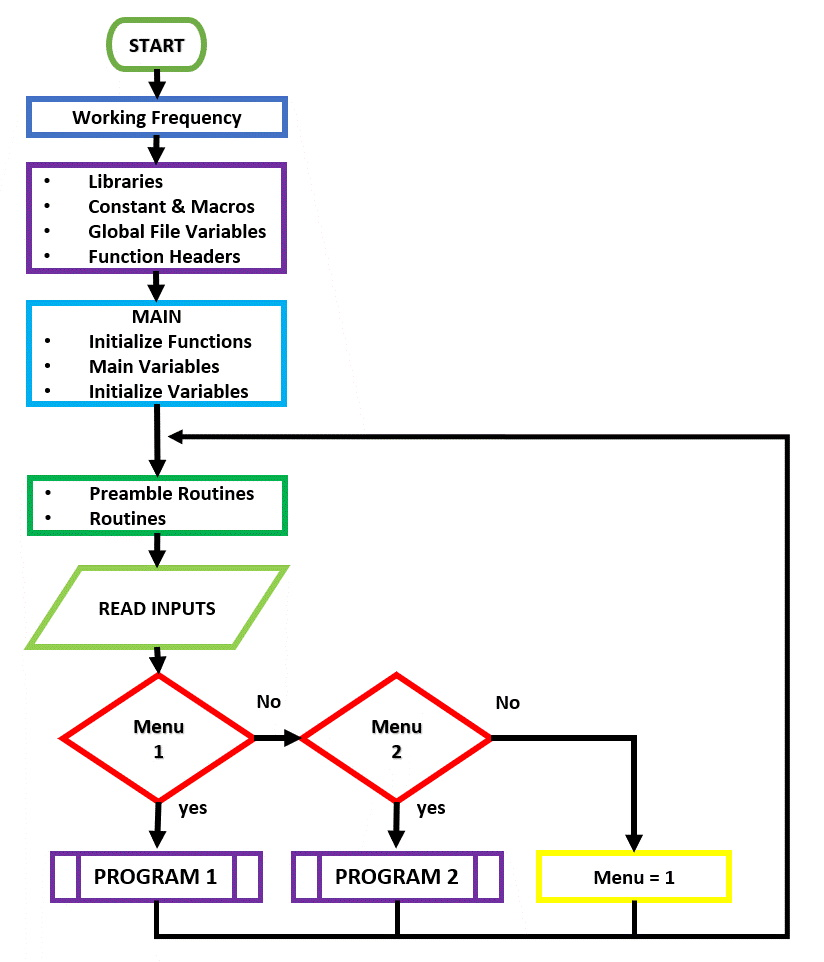
\includegraphics[scale=0.6]{./image/PESTA/flowchart/Main_Program_1.jpg}
	\caption{Estrutura do Programa}
	\label{Main_Program_1}
\end{figure}
\figurespace{.5}
O \textit{PROGRAM 1} é onde corre o programa da balança, e o \textit{PROGRAM 2} usado para calibração do \textit{Gain Factor}.
\\
\\
Todos os programas sequem uma estrutura sintática recursiva usando o seguinte modelo.
\\
\\
\begin{figure}[H]
	\centering
	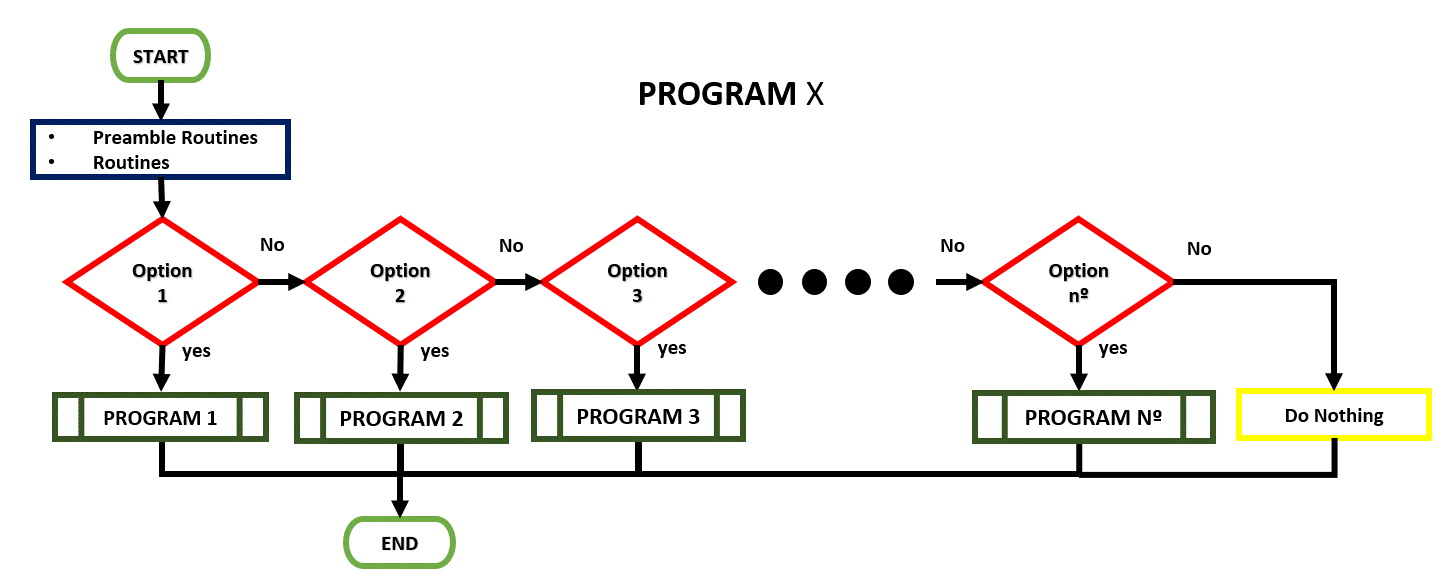
\includegraphics[scale=0.40]{./image/PESTA/flowchart/Generic_structure.jpg}
	\caption{Sintaxe Genérica dos programas}
	\label{Geneic_structure}
\end{figure}
\figurespace{.5}
Duas interrupções periódicas estão sempre a correr em \textit{background}, uma para fazer o \textit{shift} dos \textit{bit´s} da conversão \textbf{ADC} feita pelo amplificador de sinal HX711 e outra interrupção periódica de segundo em segundo usado para saltar de \textit{Menu} pelos botões.
\\
\\
\begin{minipage}{\linewidth}
\begin{minipage}{.5\linewidth}
\begin{figure}[H]
	\centering
	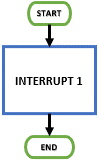
\includegraphics[scale=0.7]{./image/PESTA/flowchart/Interrupt_1.jpg}
	\caption{\textbf{ADC} conversão}
	\label{Interrupt_1}
\end{figure}
\end{minipage}
\begin{minipage}{.5\linewidth}
\begin{figure}[H]
	\centering
	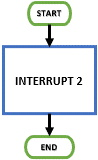
\includegraphics[scale=0.7]{./image/PESTA/flowchart/Interrupt_2.jpg}
	\caption{Saltar de \textit{Menu}}
	\label{Interrupt_2}
\end{figure}
\end{minipage}
\end{minipage}
\minipagespace{.5}
Consultar código para leitura das rotinas de interrupção nas folhas \textit{anexas}.
\\
\\
\begin{minipage}{.40\linewidth}
\begin{figure}[H]
	\flushleft
	\captionsetup{justification=raggedright,singlelinecheck=false}
	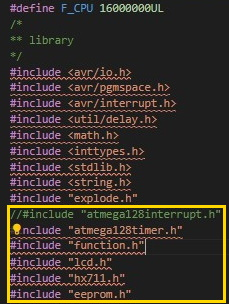
\includegraphics[scale=0.9]{./image/PESTA/Code/Livrarias.jpg}
	\caption{Livrarias}
	\label{Livrarias}
\end{figure}
\end{minipage}
\begin{minipage}{.6\linewidth}
Ao lado esta as livrarias usadas neste projeto, as que estão dentro da caixa amarela são as que foram criadas.
A filosofia usada é de criar objetos que representam o hardware para o poder manipular via código. Como se pode observar foi criado uma livraria para os temporizadores, outra paras as interrupções e \textbf{EEPROM} depois criado livrarias para os componentes externos, isto é, o \textbf{LCD} e o integrado \textbf{HX711}. \\
Uma abstração que torna simples executar qualquer algoritmo ou projeto, e isto só é possível depois de ultrapassar a barreira árdua e dolorosa de desenvolver as livrarias.
\\
\\
\\
\end{minipage}
\newpage
\section{Validação}
%%%To validate is to justify why the choices made and alternatives that could be chosen.
As escolhas feitas estão dentro dos parâmetros da oferta disponibilizada. Apenas o conhecimento adquirido ao aprofundar o funcionamento dos componentes é o ganho mais evidente, facilitando a interpretação de situações e deteção de anomalias (\textit{troubleshooting}), derivado aos custos dos materiais serem caros.\\
\\
Apostei na marca \textbf{Atmel} devido a experiência e conhecimentos já adquiridos, se aposta-se noutra marca teria de enfrentar uma curva de aprendizagem e adaptação que no final a nível de custos beneficio seria desfavorável, pelo tempo a dispensar e de ser muito trabalhoso a refazer tudo novamente noutra arquitetura.\\
\\
O sensor usado é o mais comum nesta pratica, e escolha demonstrada, o circuito de interface é indiferente a escolha apenas é baseada na sua precisão, ou seja, é de \textcolor{blue}{24} \textit{bit} enquanto o \textbf{ADC} do \textbf{MCU} de \textcolor{blue}{10} \textit{bit}.
\\
\\
\\
\subsection{Material}
Abaixo esta indicado uma tabela dos materiais usados, assim como os preços.
\\
\\
\begin{table}[H]{
		\caption{Lista de material}
		\rowcolors{3}{blue!80!yellow!50}{blue!70!yellow!40}
		\begin{tabular}{ |p{12cm}|c|p{2cm}|  }
			\hline
			\multicolumn{3}{|c|}{Lista de Material} \\
			\hline
			Peça & Quant & Preço [uni] \\
			\hline
			Fonte de alimetação 12V 1A & 1 & \EUR{3.87} \\
			Conversor DC-DC com voltímetro & 1 & \EUR{7.75} \\
			ET BASE AVR Atmega128 Board & 1 & \EUR{23.92} \\
			Test Input Board  & 1 & \EUR{3.71} \\
			Test Output Board & 1 & \EUR{3.71} \\
			IDC Socket 10 way    & 12 & \EUR{0.31} \\
			IDC Header Straight 10 way    & 12 & \EUR{0.25} \\
			Flatcable    & ? & \EUR{?} \\
			20x4 LCD Module Blue & 1 & \EUR{12.24} \\
			SparkFun Load Cell Amplifier HX711 & 1 & \EUR{13.04}   \\
			50Kg Load Cell & 1 & \EUR{12} \\
			\hline
			& \textit{total} & \EUR{86.96} \\
			\hline
		\end{tabular}
	}
	\label{material}
\end{table}


\subsection*{Testar}
Quanto a funcionalidade no seu todo a balança tem \textcolor{blue}{quatro} botões e \textcolor{blue}{três} \textit{leds} ativados, um botão para fazer o \textit{offset} no \textcolor{green}{PORTF 0}, e dois botões com dupla função, fazer \textit{reset} para \textit{default} e incrementar, outro para entrar no menu de calibração e decrementar, o \textcolor{blue}{quarto} botão é reservado para \textit{enter} e assumir o valor introduzido na calibração.\\
\\
O botão \textcolor{green}{PORTF 3} quando premido durante \textcolor{blue}{cinco} segundos faz um \textit{reset} para configuração \textit{default} depois de o \textit{led} no \textcolor{red}{PORTC 6} piscar \textcolor{blue}{quatro} vezes.\\
\\
O botão \textcolor{green}{PORTF 4} quando premido durante \textcolor{blue}{cinco} segundos entra no menu de calibração do valor do \textit{gain factor} e o \textit{led} no \textcolor{red}{PORTC 7} liga, usando os botões de incrementa e decrementar, isto é, o
\textcolor{green}{PORTF 3} e \textcolor{green}{PORTF 4} pode-se alterar esse valor.\\
\\
Para assumir o valor e sair do menu de calibração basta premir o botão colocado no \textcolor{green}{PORTF 5}. Tanto no caso de calibração ou de \textit{offset} os valores são guardados na \textbf{EEPROM} do microcontrolador, sendo que, se retirar a alimentação do circuito este não perde os valores e o \textit{led} \textcolor{red}{PORTC 5} permanece ligado.
\\
\\
%%%%%%%%%%%%%%%%%%%%%%%%%%%%%%%%%%%%%%%%%%%%%%%%%%%%%%%%%%%%%%%%
\begin{comment}
Sem contar com as despesas no equipamento para a programação do hardware que em principio só se gasta uma vez, isto é, se não se estragar. No caso do programador \textbf{Atmel-ICE} pode custar até \EUR{185.55}.\\
\\
É de ter em conta que os preços são \textbf{PVP}, que no caso se for preços comerciais são dez vezes inferior, e se for para produção em grande escala também tem descontos por quantidade.\\
$\begin{array}{l l l}
\text{Média} & & \\
\overline{x} & = & \frac{1}{n}\sum_{i=1}^n x_i
\end{array}$
MEMS devices and structures are fabricated using conventional integrated circuit process techniques, such as lithography, deposition, and etching, together with a broad range of specially developed micromachining techniques. \cite{book-9}
The three essential elements in conventional silicon processing are deposition, lithography, and etching. \cite{book-9}
Sensitivity,Long-Term Drift e Temperature Effects (Span temperature hysteresis).
\end{comment}
%%%%%%%%%%%%%%%%%%%%%%%%%%%%%%%%%%%%%%%%%%%%%%%%%%%%%%%%%%%%%%%%
	\newpage
	\chapter{Conclusão}
%\setcounter{section}{0}
%%%%%%%%%%%%%%%%%%%%%%%%%%%%%%%%%%%%%%%%%%%%%%%%%%%%%%%%%%%%%%%%
\qquad O futuro do trabalho passa por adquirir novas competências, e conseguir adaptação as novas tendências, a procura de oportunidades e valorização pessoal uma mais valia. Já foi demonstrado que é importante desenvolvermos tanto as nossas metodologias de trabalho como a experiência para estarmos preparados para enfrentar os desafios que possam surgir. \\
\\
Ninguém sabe o futuro, muito menos o imprevistos, cabe as novas gerações decidir, a liberdade acho que é algo que todos desejam, a estabilidade e segurança, mas não só depende de nós, o planeta terra, a galáxia e o universo tem palavra soberana.\\
\\
Considero a humildade e gratidão um atributo fundamental, saber que estamos sujeitos a forças maiores e respeitar essas fronteiras, historicamente isso foi comprovado vezes sem conta, e hoje é outra prova disso, como a pandemia.\\
\\
Gerações após gerações existe uma concentração tremenda muito focada com uma visão míope, um convite para o desastre. Sabe-se lá se temos cura. No entanto temos que ter esperança que haja visão e iluminação.
Esta conversa até parece religiosa, mas nada disso.\\
\\
Ainda muitas conclusões pode-se tirar acerca do futuro do trabalho e marketing pessoal, que não entra nos parâmetros deste relatório e discussão, o desenvolvimento é uma forma de enriquecimento mais rápido e eficaz, com contornos sociais complicados, da a entender que vai haver um excesso de produção sem clientes á vista, um problema de reciclagem e sobrevivência, talvez devia haver uma preocupação na  regulamentação.\\
\\
O ensino talvez esta a ficar desadequado para nossos tempos, não incluindo as ferramentas necessárias na formação e treino, o tempo de retenção dos estudantes excessivo, que provoca colisões entre gerações, especialmente num país pequeno com uma cultura estática, sendo quase impossível obter os resultados esperados caindo na decadência social e económica no seu geral, etc, etc, etc.\\
\\
No meu ver \textcolor{green}{Portugal} deixou de ser um país mas uma fábrica, as competências uma forma de sobreviver no sentido de estar numa escala mais favorável, dai que a solução de mudar para uma sociedade onde o valor individual depende das competências origina a juventude fugir deste sistema instalado.\\
\\
Abaixo link de apanhado de dados utilizados para este relatório:\\ \textcolor{green}{\small [ https://padlet.com/sergio1020881/xih48fe75koesxdg ]}

	\newpage
	%%%%%%%%%%%%%%%%%%%%%%%%%%%%%%%%%%%%%%%%%%%%%%%%%%%%%%%%%%%%
	\setstretch{.8}
	%%%END%%%
\appendix
%%%%%%%%%%%%%%%%%%%%%%%%%%%%%%%%%%%%%%%%%%%%%%%%%%%%%%%%%%%%%%%%
%\chapter{\Large{Definições}}
%\vspace{0.2cm}
%%%%%%%%%%%%%%%%%%%%%%%%%%%%%%%%%%%%%%%%%%%%%%%%%%%%%%%%%%%%%%%%
\begin{minipage}[t]{0.55\linewidth}
	\begin{definition}
		Capacit\^{a}ncia
		\begin{flalign*}
			Q_c(t) =& \int^t i(t) \quad dt & \\
			=& Q_c(0^-)+\int_{0^-}^t i(t) \quad dt & \\
			V_c(t) =& \frac{Q_c(t)}{C} & \\
			=& \frac{1}{C} \quad \int^t i_c(t) \quad dt & \\
			=& \frac{Q_c(0^-)}{C} + \frac{1}{C} \quad \int_0^t i_c(t) \quad dt & \\
			=& V(0^-) + \frac{1}{C} \quad \int_0^t i_c(t) \quad dt & \\
			i_c(t) =& C \quad \dfrac{d V_c(t)}{dt} & \\
			W = & \frac{1}{2} \; C \; V^{2} &
		\end{flalign*}\par
	\end{definition}
\end{minipage}
%
\begin{minipage}[t]{0.55\linewidth}
	\begin{definition}
		Indut\^{a}ncia
		\begin{flalign*}
			\psi_L(t) =& \int^t V_L(t) \quad dt & \\
			=& \psi_L(0^-)+\int_{0^-}^t V_L(t) \quad dt & \\
			V_L(t) =& L \quad \dfrac{d i_L(t)}{dt} & \\
			i_L(t) =& \frac{\psi_L(t)}{L} & \\
			=& \frac{1}{L} \quad \int^t V_L(t) \quad dt & \\
			=& \frac{\psi_L(0^-)}{L} + \frac{1}{L} \quad \int_0^t V_L(t) \quad dt &  \\
			=& i_L(0^-) + \frac{1}{L} \quad \int_0^t V_L(t) \quad dt & \\
			W = & \frac{1}{2} \; L \; i^{2} &
		\end{flalign*}\par
	\end{definition}
\end{minipage}
\vspace{2cm}
\par
\begin{minipage}[t]{0.55\linewidth}
	\begin{definition}
		Resist\^{e}ncia
		\begin{flalign*}
			V_R(t) = \; & R \quad i_R(t) & \\
			i_R(t) = \; & \frac{V_R(t)}{R} & \\
			P \; = \; & R i^{2} & \\
			P \; = \; & \frac{U^{2}}{R} & \\
			W \; = \; & P \; \Delta t &
		\end{flalign*}\par
	\end{definition}
\end{minipage}
%
\begin{minipage}[t]{0.55\linewidth}
	\begin{definition}
		Valor M\'{e}dio
		\begin{flalign*}
			X_{av} =& \frac{1}{T} \; \int_0^T X(t) dt &
		\end{flalign*}\par
	\end{definition}
	%
	\begin{definition}
		Valor Eficaz
		\begin{flalign*}
			X_{ef} =& \sqrt{ \frac{1}{T} \; \int_0^T \overset{\text{2}}{X(t)} dt } &
		\end{flalign*}\par
	\end{definition}
\end{minipage}
%%%%%%%%%%%%%%%%%%%%%%%%%%%%%%%%%%%%%%%%%%%%%%%%%%%%%%%%%%%%%%%%

%\newpage
\chapter{Física}
%%%%%%%%%%%%%%%%%%%%%%%%%%%%%%%%%%%%%%%%%%%%%%%%%%%%%%%%%%%%%%%%
\begin{minipage}[c]{\linewidth}
	\section*{Força  [N] [Kgf]}
	\Large
	$\begin{array}{ l l l l l }
		\sum F_{(t)} & = & M \; a_{(t)} & = & M \; \ddot{x}_{(t)}
	\end{array}$
	\newline
	\newline
	$\begin{array}{ l l l }
		\sum F_{R} & = & \sum F_{action} \; - \; \sum F_{reaction}
	\end{array}$
	\newline
	\newline
	$\begin{array}{ l l l }
		f_{(t)} & = & -K \; x_{(t)} \\
		f_{(t)} & = & -B \; \dot{x}_{(t)}
	\end{array}$
	\newline
	\newline
	%%%There are only forces if there is a physical object subject to them.
\end{minipage}
\newline
\vspace{.6cm}
\newline
\begin{minipage}[c]{\linewidth}
	\section*{Torque [N.m]}
	\Large
	$\begin{array}{ l l l l l }
		\sum T_{(t)} & = & J \; \gamma_{(t)} & = & M \; \ddot{\theta}_{(t)}
	\end{array}$
	\newline
	\newline
	$\begin{array}{ l l l }
		\sum T_{R} & = & \sum T_{action} \; - \; \sum T_{reaction}
	\end{array}$
	\newline
	\newline
	$\begin{array}{ l l l }
		T_{(t)} & = & -K \; \theta_{(t)} \\
		T_{(t)} & = & -B \; \dot{\theta}_{(t)} \\
		T & = & F \times r
	\end{array}$
	\newline
	\newline
	%%%Never mix potatoes with bananas.
\end{minipage}
\newline
\vspace{.6cm}
\newline
\begin{minipage}[c]{.5\linewidth}
	\section*{Energia [Joule]}
	\vspace{.1cm}
	\Large
	$\begin{array}{ l l l }
		W & = & F \; d \\
		W & = & P \; \Delta t \\
		E & = & M \; C^{2}
	\end{array}$
\end{minipage}
\begin{minipage}[c]{.5\linewidth}
	\begin{figure}[H]
		\flushleft
		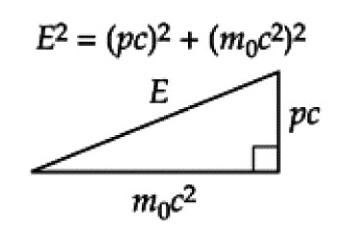
\includegraphics[scale=0.6]{./image/PESTA/general/Einstein.jpg}
		\caption*{\cite{book-2}}
		\label{Einstein}
	\end{figure}
\end{minipage}
\newline
\vspace{.6cm}
\newline
\begin{minipage}[!b]{.5\linewidth}
	\section*{Energia Cinética [Joule]}
	\Large
	$\begin{array}{ l l l }
		E_{c} & = & \frac{1}{2} \; m \; v^{2}
	\end{array}$
\end{minipage}
\begin{minipage}[!b]{.5\linewidth}
	\section*{Energia Potencial [Joule]}
	\Large
	$\begin{array}{ l l l }
		E_{p} & = & \; m \; g \; h
	\end{array}$
\end{minipage}
\newline
\vspace{.6cm}
\newline
\begin{minipage}[l]{\linewidth}
	\section*{Energia Térmica}
	\Large
	$\begin{array}{ l l l l }
		Q - Heat \quad energy & & & \\
		Q_{(t)} - temperature & & & \\
		R - heat \quad resistance & & & \\
		& Q & = & \frac{Q_{1(t)} - Q_{2(t)}}{R}
	\end{array}$
\end{minipage}
%%%%%%%%%%%%%%%%%%%%%%%%%%%%%%%%%%%%%%%%%%%%%%%%%%%%%%%%%%%%%%%%
%%%%%%%%%%%%%%%%%%%%%%%%%%%%%%%%%%%%%%%%%%%%%%%%%%%%%%%%%%%%%%%%
%%%%%%%%%%%%%%%%%%%%%%%%%%%%%%%%%%%%%%%%%%%%%%%%%%%%%%%%%%%%%%%%
%%%%%%%%%%%%%%%%%%%%%%%%%%%%%%%%%%%%%%%%%%%%%%%%%%%%%%%%%%%%%%%%
\begin{comment}
\newline
\vspace{1cm}
\newline
$\frac{A \times B}{C}\times D \approx E$,
\newline
\begin{minipage}{0pt}
	$$\begin{array}{l | l}
		\text{Média aritmetica dados classificados} & \text{Variância de uma amostra dados classificados} \\
		\overline{x} = \frac{1}{n}\sum_{i=1}^cx_in_i = \sum_{i=1}^cx_if_i & s^2 = \frac{1}{n-1}\sum_{i=1}^c (x_i-\bar{x})^2 n_i
	\end{array}$$
\end{minipage}
\newline
\vspace{1cm}
\newline
$IC_{1-\alpha}=\left[ A, B\right]$ ; para $1-\alpha = 0.95$, $\alpha=0.05$, $\frac{\alpha}{2}=0.025$
\newline
\vspace{1cm}
\newline
Zona critica $Z_c=Z_{1-\frac{\alpha}{2}}=\Phi^{-1}(0.975) \cong 1.96$
\newline
\vspace{1cm}
\newline
$P\left( A \leqslant \mu \leqslant B \right) = 1-\alpha$ \\
$\triangle=Z_c\times\frac{\delta}{\sqrt{n}}$ \\
$A = \bar{x}-\triangle \qquad and \qquad B = \bar{x}+\triangle$ \\
$\therefore$\\
$IC_{A_{0.95}}=\left[ \; 18.8877 \: , \: 21.1956 \; \right]$ \hspace{1cm} and \hspace{1cm} $IC_{B_{0.95}}=\left[ \; 20.4519 \: , \: 22.6314 \; \right]$
\newline
\vspace{1cm}
\newline
$\left[ \; \mu \; \right]$
\newline
\vspace{1cm}
\newline
$\bar{y}_{A_0}$ = 6,6111 \qquad $\bar{y}_{B_0}$ = 7,5111 \qquad $n=90$ \\
$\delta_A$ = 2,3112 \qquad $\delta_B$ = 2,5140
\newline
\vspace{1cm}
\newline
$P(Y_A < 6)=P(Y_A \leqslant 5)=F_{i_B}(5) \cong 0,3677 $  \quad e \quad $P(Y_B < 6)=P(Y_B \leqslant 5)=F_{i_B}(5) \cong 0,2444$ \\
\newline
\vspace{1cm}
\newline
$\hat{P_A}-\hat{P_B} \sim N \left( p_A - p_B ; \frac{p_A\:q_A}{n_A} + \frac{p_B\:q_B}{n_B}\right)$ \hspace{1cm}
$\triangle=z_{(1-\frac{\alpha}{2})} \;\sqrt{\frac{\hat{p_A} \: \hat{q_A}}{n_A}+\frac{\hat{p_B} \: \hat{q_B}}{n_B}}$ \hspace{1cm} $q=(1-p)$
\newline
\vspace{1cm}
\newline
$IC_{97\%}(\hat{P_A}-\hat{P_B})=\left[(\hat{p_A}-\hat{p_B})-\triangle \: ; \: (\hat{p_A}-\hat{p_B})+\triangle \right]$
\newline
\vspace{1cm}
\newline
$\hat{P_A}-\hat{P_B} \sim N \left( 0,1233 \; ; \; 0,02788\right)$ \hspace{1cm}
$z_{(1-\frac{\alpha}{2})}=\phi^{-1}(0,985)=2,1701$
\newline
\vspace{1cm}
\newline
Recorrendo a calculadora casio $fx-9860GII$ :
\newline
\vspace{1cm}
\newline
$\triangle= InvNorm(0.985)\sqrt{\frac{0.3677(1-0.3677)}{90}+\frac{0.2444(1-0.2444)}{90}}\: \cong \:0.3677$
\\
$\therefore$
\\
$IC_{97\%}(\hat{P_A}-\hat{P_B})=\left[ \; (\hat{p_A}-\hat{p_B}) \:-\: 0,3624 \: ; \: (\hat{p_A}-\hat{p_B}) \:+\: 0,3624 \; \right]$
\newline
\vspace{1cm}
\newline
\begin{minipage}[l]{0pt}
	$$\left\lbrace\begin{array}{l}
		H_0: \quad \mu_A-\mu_B=0 \\
		\\
		H_1: \quad \mu_A-\mu_B<0
	\end{array}\right.$$
\end{minipage}
\newline
\vspace{1cm}
\newline
\begin{minipage}[l]{0pt}
	$$\left\lbrace\begin{array}{c}
		\mu \;=\; 0 \\
		\delta \;=\; s \\
	\end{array}\right.$$
\end{minipage}
\hspace{3cm} $\Longrightarrow$ \hspace{1cm}
\begin{minipage}[l]{0pt}
	\[\bar{X}=\bar{X}_A-\bar{X}_B \quad \backsim N \left( 0\:,\: \frac{\delta_A^2}{n_A}+\frac{\delta_B^2}{n_B} \right) \quad ; \quad \frac{\delta_A^2}{n_A}+\frac{\delta_B^2}{n_B}\;\cong0.6558 \]
\end{minipage}
\newline
\vspace{1cm}
\newline
$P(\bar{X}_{H_0} \leqslant C)=0.05 \quad \implies \quad RC_X\left] -\infty \:,\: -1.332 \right] \qquad \bar{x}_A-\bar{x}_B=-1.5 \in RC_X $
\newline
\vspace{1cm}
\newline
\begin{minipage}[l]{0pt}
	\[  z_0\:=\: \frac{\bar{x}_A-\bar{x}_B}{\sqrt{\frac{\delta_A^2}{n_A}+\frac{\delta_B^2}{n_B}}}\:\cong\: -1.8523 \qquad
	RC_z \:=\: \left] -\infty \:,\: -1.6448 \right]  \qquad
	pvalue \:=\: P(Z<z_0) \:=\: 0.032 \]
\end{minipage}
\newline
\vspace{1cm}
\newline
\hspace*{5cm} \underline{Condição NEE:}\\
\begin{minipage}[l]{0pt}
	$$\left\lbrace\begin{array}{c}
		\mu \;=\; 0 \\
		\delta \;=\; s \\
	\end{array}\right.$$
\end{minipage}
\hspace{3cm} $\Longrightarrow$ \hspace{1cm}
\begin{minipage}[l]{0pt}
	\[ \bar{Y}=\bar{Y_A}-\bar{Y_B} \quad \backsim N \left( 0\:,\: \frac{\delta_A^2}{n_A}+\frac{\delta_B^2}{n_B} \right) \quad ; \quad \frac{\delta_A^2}{n_A}+\frac{\delta_B^2}{n_B} \; \cong 0.1296 \]
\end{minipage}
\newline
\vspace{1cm}
\newline
$P(\bar{Y}_{H_0} \leqslant C)=0.05 \quad \implies \quad RC_Y\left] -\infty \:,\: -0.5921 \right] \qquad \bar{y}_A-\bar{y}_B=-0.9 \in RC_Y $
\newline
\vspace{1cm}
\newline
\begin{minipage}[l]{0pt}
	\[  z_0\:=\: \frac{\bar{y}_A-\bar{y}_B}{\sqrt{\frac{\delta_A^2}{n_A}+\frac{\delta_B^2}{n_B}}}\:\cong\: -2.5 \qquad
	RC_z \:=\: \left] -\infty \:,\: -1.6448 \right]  \qquad
	pvalue \:=\: P(Z<z_0) \:=\: 0.0062 \]
\end{minipage}
\newline
\vspace{1cm}
\newline
\begin{minipage}[l]{0pt}
	$$\left\lbrace\begin{array}{l}
		H_0: X \backsim N (20.0417\;,\;6.4494^2) \\
		\\
		H_1: X \nsim N (20.0417\;,\;6.4494^2)
	\end{array}\right.$$
\end{minipage}
\newline
\vspace{1cm}
\newline
\hspace*{5cm} \underline{NEE Região B:} \\
\begin{minipage}[l]{0pt}
	$$\left\lbrace\begin{array}{l}
		H_0: X \backsim N (7.5111\;,\;2.5140^2) \\
		\\
		H_1: X \nsim N (7.5111\;,\;2.5140^2)
	\end{array}\right.$$
\end{minipage}
\newline
\vspace{1cm}
\newline
$q_0=\sum_{i=1}^n \frac{(n_i-e_i)^2}{e_i} \;\backsim\; \chi_{(k-m-1)}^2$
\newline
\vspace{1cm}
\newline
$RC_{\chi^2}=\left[ \: InvChiCD(0.05,5) \:,\: +\infty \; \right] \quad \rightarrow \quad RC_{\chi_2}=\left[ \: 11.0705 \:,\: +\infty \; \right]$
\newline
\vspace{1cm}
\newline
$q_0=8.5532$ < 11.0705
\newline
\vspace{1cm}
\newline
$\left[ \; \mu \; \right]$
\newline
\vspace{1cm}
\newline
$\bar{y}_{A_0}$ = 6,6111 \qquad $\bar{y}_{B_0}$ = 7,5111 \qquad $n=90$ \\
$\delta_A$ = 2,3112 \qquad $\delta_B$ = 2,5140
\newline
\vspace{1cm}
\newline
$P(Y_A < 6)=P(Y_A \leqslant 5)=F_{i_B}(5) \cong 0,3677 $  \quad e \quad $P(Y_B < 6)=P(Y_B \leqslant 5)=F_{i_B}(5) \cong 0,2444$
\newline
\vspace{1cm}
\newline
$\hat{P_A}-\hat{P_B} \sim N \left( p_A - p_B ; \frac{p_A\:q_A}{n_A} + \frac{p_B\:q_B}{n_B}\right)$ \hspace{1cm}
$\triangle=z_{(1-\frac{\alpha}{2})} \;\sqrt{\frac{\hat{p_A} \: \hat{q_A}}{n_A}+\frac{\hat{p_B} \: \hat{q_B}}{n_B}}$ \hspace{1cm} $q=(1-p)$
\newline
\vspace{1cm}
\newline
$IC_{97\%}(\hat{P_A}-\hat{P_B})=\left[(\hat{p_A}-\hat{p_B})-\triangle \: ; \: (\hat{p_A}-\hat{p_B})+\triangle \right]$
\newline
\vspace{1cm}
\newline
$\hat{P_A}-\hat{P_B} \sim N \left( 0,1233 \; ; \; 0,02788\right)$ \hspace{1cm}
$z_{(1-\frac{\alpha}{2})}=\phi^{-1}(0,985)=2,1701$
\newline
\vspace{1cm}
\newline
Recorrendo a calculadaora casio $fx-9860GII$ :
\newline
\vspace{1cm}
\newline
$\triangle= InvNorm(0.985)\sqrt{\frac{0.3677(1-0.3677)}{90}+\frac{0.2444(1-0.2444)}{90}}\: \cong \:0.3677$
\\
$\therefore$
\\
$IC_{97\%}(\hat{P_A}-\hat{P_B})=\left[ \; (\hat{p_A}-\hat{p_B}) \:-\: 0,3624 \: ; \: (\hat{p_A}-\hat{p_B}) \:+\: 0,3624 \; \right]$
\newline
\vspace{1cm}
\newline
\begin{minipage}[l]{0pt}
	$$\left\lbrace\begin{array}{l}
		H_0: \quad \mu_A-\mu_B=0 \\
		\\
		H_1: \quad \mu_A-\mu_B<0
	\end{array}\right.$$
\end{minipage}
\newline
\vspace{1cm}
\newline
\begin{minipage}[l]{0pt}
	$$\left\lbrace\begin{array}{c}
		\mu \;=\; 0 \\
		\delta \;=\; s \\
	\end{array}\right.$$
\end{minipage}
\hspace{3cm} $\Longrightarrow$ \hspace{1cm}
\begin{minipage}[l]{0pt}
	\[\bar{X}=\bar{X}_A-\bar{X}_B \quad \backsim N \left( 0\:,\: \frac{\delta_A^2}{n_A}+\frac{\delta_B^2}{n_B} \right) \quad ; \quad \frac{\delta_A^2}{n_A}+\frac{\delta_B^2}{n_B}\;\cong0.6558 \]
\end{minipage}
\newline
\vspace{1cm}
\newline
$P(\bar{X}_{H_0} \leqslant C)=0.05 \quad \implies \quad RC_X\left] -\infty \:,\: -1.332 \right] \qquad \bar{x}_A-\bar{x}_B=-1.5 \in RC_X $
\newline
\vspace{1cm}
\newline
\begin{minipage}[l]{0pt}
	\[  z_0\:=\: \frac{\bar{x}_A-\bar{x}_B}{\sqrt{\frac{\delta_A^2}{n_A}+\frac{\delta_B^2}{n_B}}}\:\cong\: -1.8523 \qquad
	RC_z \:=\: \left] -\infty \:,\: -1.6448 \right]  \qquad
	pvalue \:=\: P(Z<z_0) \:=\: 0.032 \]
\end{minipage}
\newline
\vspace{1cm}
\newline
\hspace*{5cm} \underline{Condição NEE:}\\
\begin{minipage}[l]{0pt}
	$$\left\lbrace\begin{array}{c}
		\mu \;=\; 0 \\
		\delta \;=\; s \\
	\end{array}\right.$$
\end{minipage}
\hspace{3cm} $\Longrightarrow$ \hspace{1cm}
\begin{minipage}[l]{0pt}
	\[ \bar{Y}=\bar{Y_A}-\bar{Y_B} \quad \backsim N \left( 0\:,\: \frac{\delta_A^2}{n_A}+\frac{\delta_B^2}{n_B} \right) \quad ; \quad \frac{\delta_A^2}{n_A}+\frac{\delta_B^2}{n_B} \; \cong 0.1296 \]
\end{minipage}
\newline
\vspace{1cm}
\newline
$P(\bar{Y}_{H_0} \leqslant C)=0.05 \quad \implies \quad RC_Y\left] -\infty \:,\: -0.5921 \right] \qquad \bar{y}_A-\bar{y}_B=-0.9 \in RC_Y $
\newline
\vspace{1cm}
\newline
\begin{minipage}[l]{0pt}
	\[  z_0\:=\: \frac{\bar{y}_A-\bar{y}_B}{\sqrt{\frac{\delta_A^2}{n_A}+\frac{\delta_B^2}{n_B}}}\:\cong\: -2.5 \qquad
	RC_z \:=\: \left] -\infty \:,\: -1.6448 \right]  \qquad
	pvalue \:=\: P(Z<z_0) \:=\: 0.0062 \]
\end{minipage}
\newline
\vspace{1cm}
\newline
\begin{minipage}[l]{0pt}
	$$\left\lbrace\begin{array}{l}
		H_0: X \backsim N (20.0417\;,\;6.4494^2) \\
		\\
		H_1: X \nsim N (20.0417\;,\;6.4494^2)
	\end{array}\right.$$
\end{minipage}
\newline
\vspace{1cm}
\newline
\hspace*{5cm} \underline{NEE Região B:} \\
\begin{minipage}[l]{0pt}
	$$\left\lbrace\begin{array}{l}
		H_0: X \backsim N (7.5111\;,\;2.5140^2) \\
		\\
		H_1: X \nsim N (7.5111\;,\;2.5140^2)
	\end{array}\right.$$
\end{minipage}
\newline
\vspace{1cm}
\newline
$q_0=\sum_{i=1}^n \frac{(n_i-e_i)^2}{e_i} \;\backsim\; \chi_{(k-m-1)}^2$
\newline
\vspace{1cm}
\newline
$RC_{\chi^2}=\left[ \: InvChiCD(0.05,5) \:,\: +\infty \; \right] \quad \rightarrow \quad RC_{\chi_2}=\left[ \: 11.0705 \:,\: +\infty \; \right]$
\newline
\vspace{1cm}
\newline
$q_0=8.5532$ < 11.0705
\newline
\vspace{1cm}
\newline
\begin{minipage}[l]{0pt}
	$$\left\lbrace\begin{array}{l}
		H_0: \bar{X}_{H_0} \backsim N (0 \;,\; 0.6558) \\
		\\
		H_1: \bar{X}_{H_1} \backsim N (-1.5 \;,\; 0.6558)
	\end{array}\right.$$
\end{minipage}
\newline
\vspace{1cm}
\newline
$\beta=P(Aceitar H_0 | H_0 é Falsa)$ \\
$\beta=(\bar{X}_{H_1} \:>\: -1.332)$	\\
$\beta=NormCD(-1.332,99999999,\sqrt{0.6558},-1.5)=0.4178$ \\
Potência do teste \\
$1-\beta=P(Rejeitar H_0 | H_0 é Falsa)=0.5822$
\newline
\vspace{1cm}
\newline
NEE Região B:\\
\begin{minipage}[l]{0pt}
	$$\left\lbrace\begin{array}{l}
		H_0: \bar{Y}_{H_0} \backsim N (0 \;,\; 0.1296) \\
		\\
		H_1: \bar{Y}_{H_1} \backsim N (-0.9 \;,\; 0.1296)
	\end{array}\right.$$
\end{minipage}
\newline
\vspace{1cm}
\newline
$\beta=P(Aceitar H_0 | H_0 é Falsa)$ \\
$\beta=(\bar{Y}_{H_1} \:>\: -0.5921)$	\\
$\beta=NormCD(-0.5921,99999999,\sqrt{0.1296},-0.9)=0.1962$ \\
Potência do teste \\
$1-\beta=P(Rejeitar H_0 | H_0 é Falsa)=0.8038$
\newline
\vspace{1cm}
\newline
$\chi^2$
\end{comment}
%%%%%%%%%%%%%%%%%%%%%%%%%%%%%%%%%%%%%%%%%%%%%%%%%%%%%%%%%%%%%%%%

%\newpage
%%\renewcommand{\labelitemi}{$\blacksquare$}
\begin{center}\textbf{\large Competências Consideradas no Estudo OCDE}
%%%\begin{center}\textbf{\large Competências Consideradas no Estudo OCDE \cite{article_1}}
\end{center}
\begin{minipage}[t]{.5\linewidth}
\qquad \textbf{Competências Cognitivas:}
\begin{itemize}
\setlength\itemsep{-1em}
\item Numeração:\\
- Números\\
- Contar\\
- Aritmética\\
\item Literacia:\\
- Falar, Ler, Escrever, Línguas\\
\item Resolução de problemas:\\
- Raciocínio\\
- Lógica\\
- Silogismo\\
- Método Socrático\\
- Critica Interrogativa\\
- etc
\end{itemize}
\qquad \textbf{Competências Socioeconómicas:}
\begin{itemize}
\setlength\itemsep{-1em}
\item Identidade\\
\item Formação Académica:\\
\item Experiência Profissional
\end{itemize}
\qquad \textbf{Personalidade:}\\
\hspace*{1cm}- Facilidade de adaptação\\
\hspace*{1cm}- Facilidade de aprendizagem\\
\hspace*{1cm}- Imaginação\\
\hspace*{1cm}- Estabilidade Emocional\\
\end{minipage}
\begin{minipage}[t]{.5\linewidth}
\qquad \textbf{Competências Operacionais:}
\begin{itemize}
\setlength\itemsep{-0.8em}
\item Gestão e Comunicação:\\
- Planear, Organizar, Controlar, etc\\
- Comunicação formal e informal\\
\item Contabilidade e Vendas:\\
- Marketing Mix\\
- Analise de Parêto\\
- etc\\
\item Organização Pessoal:\\
- Diagrama de Gantt\\
- Analise de Parêto\\
- etc\\
\item Numeração Avançada:\\
- Aritmética, Álgebra, Geometria\\
- Trigonometria, Cálculos\\
- Sistemas Dinâmicos\\
- Estatística\\
- etc\\
\item Tecnologias de informação e comunicação:\\
- Computadores, Telemóvel\\
- Internet, e-mail\\
- Programação\\
- Telecomunicações\\
- etc\\
\end{itemize}
\end{minipage}

%\newpage
%\section{Plano de desenvolvimento pessoal de competências}
\qquad O meu plano de desenvolvimento pessoal, passa por obter mais formação e aprender com pessoas com mais experiência em diversas áreas, que é exatamente o que estou a fazer frequentando o curso de Engenharia Eletrotécnica e de Computadores no \textcolor{gray}{I.S.E.P}.\\
Esta disciplina em particular é uma forma de poder enriquecer minhas competências e metodologias de Gestão, e perceber as restantes matérias abordadas que compõem o \textcolor{blue}{Comportamento Organizacional}.\\
\begin{minipage}{8cm}
	\textbf{Metodologias da gestão}: \\
	%%%\textbf{Metodologias da gestão}: \cite{book_9}\\
	\\
	\begin{minipage}{3.1cm}
		Instrumental
		\begin{enumerate}
			\setlength\itemsep{-0.3em}
			\item Planear
			\item Organizar
			\item Controlar\\
		\end{enumerate}
	\end{minipage}
	\begin{minipage}{4cm}
		Comportamental
		\begin{enumerate}
			\setlength\itemsep{-0.3em}
			\item Liderança
			\item Comunicação
			\item Motivação
			\item Tomada de decisão
		\end{enumerate}
	\end{minipage}
\end{minipage}
\begin{minipage}{9cm}
\begin{figure}[H]
	\flushleft
	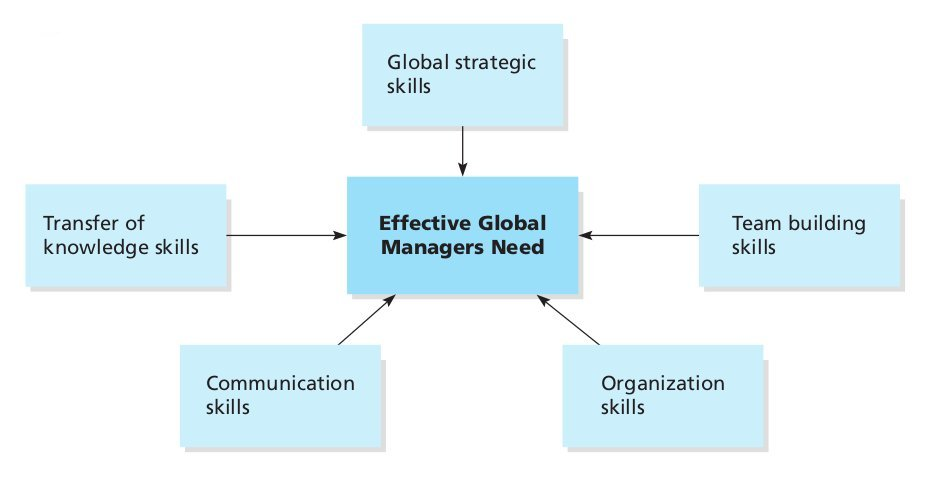
\includegraphics[scale=0.3]{./image/CORGA/Skills/Managerial_Skills_for_the_Global_Marketplace.jpg}
	\caption{Competências de Gestão.}
	%%%\caption{Competências de Gestão. \cite{book_6}}
\end{figure}
\end{minipage}
\\
\\
No entanto por enquanto minha missão é concluir a formação, e ao mesmo tempo melhorar um conjunto de ferramentas e métodos de trabalho para que seja estável e eficaz de forma a poder resolver os problemas que possa ter que enfrentar com facilidade, e eventualmente realizar alguns projetos pessoais. \\
\\
\newpage
\subsection{Análise S.W.O.T Pessoal}
\qquad Neste contexto de plano de desenvolvimento a análise \textcolor{blue}{SWOT} também pode ser uma ferramenta útil de forma a nos indicar qual os comportamentos que poderá ser melhorado ou alterado.
\newline
\newline
\fbox{
\begin{minipage}[t]{\linewidth}
\begin{itemize}
	\setlength\itemsep{-0.85em}
	\item \textcolor{purple}{I}nterno
	\begin{itemize}
		\setlength\itemsep{-0.3em}
		\item \textcolor{orange}{S}trength (forças) \\
		- Numeração, Literacia Bilingue, Resolução de Problemas \\
		- Formação Académica, Experiência Profissional \\
		- Facilidade de Adaptação e aprendizagem, Imaginação \\
		- Gestão e Comunicação, Organização Pessoal \\
		- Numeração Avançada, Tecnologias de informação e comunicação. \\
		- Estabilidade Emocional \\
		- Empatia, Método Cientifico
		\item \textcolor{orange}{W}eakness (fraquezas) \\
		- Contabilidade e Vendas \\
		- Direto, Crítico, Detesto desigualdade e injustiças \\
		- Frontal com contradições \\
		- "Dente por dente e olho por olho" \\
		- Anti-Dogma
	\end{itemize}
	\item \textcolor{purple}{E}xterno
	\begin{itemize}
		\setlength\itemsep{-0.3em}
		\item \textcolor{orange}{O}pportunity (oportunidades) \\
		- Nenhum
		\item \textcolor{orange}{T}hreats (ameaças) \\
		- Cultura Portuguesa \\
		- Sistema Político-Social \\
		- Racismo
	\end{itemize}
\end{itemize}
\end{minipage}
} \vspace{.2cm}

Algumas explicações de personalidade descrevo no caso de quando se diz "dente por dente e olho por olho", muitas das vezes tem interpretação errada, pois concluem que existiria apenas cegos após alguns tempos, mas sendo uma metáfora, sabe-se que ninguém vai andar a cegar uns aos outros sem motivo e são circunstancias de saber individual, mas deve ser percebido no aspeto em que uma pessoa que é honesta merece honestidade, e uma humilde humildade, e pelo verso um mentiroso aldrabado, e assassino deve ser morto, este procedimento leva com que o bem vence sempre, isto é lógico e citações milenares de certa forma condiz neste caso. Que levanta também a questão da veracidade da perceção, na qual muito cuidado é exigido. \\
Dai que certas pessoas quando estão a ser irónicas, acabam dececionados com as reações esperadas, podendo entrar em ciclos viciosos que só vão agravando.\\
\\
Quanto ao método cientifico nos diz que se um acontecimento se repete nas mesmas circunstâncias e nunca se altera é considerado facto ou lei ou teoria, é uma arte de reconhecer padrões. Também nós ensina que os conhecimentos estão sempre abertos ao escrutínio e se houver prova que refuta a teoria esta deixa de o ser, ou seja, é tentar representar a realidade observada por modelos racionais e matemáticos, as ferramentas que estão ao nosso dispor, já que não existe melhor. \\
\\
Acho que esta análise seria mais prudente se fosse feito por uma perspetiva de terceiros, pois nos faria refletir nossas próprias preposições podendo ser reforçado ou até alterado.
\subsection{Curriculum Vitae}
\qquad Curriculum vitae significa "percurso de vida" \; em latim, ao primeiro era pouco conhecido e pouco utilizado, ou reservado apenas a uma fração da população ativa, principalmente aos jovens diplomados ou aos quadros que mudavam de "situação". No entanto os tempos mudaram devido a instabilidade e mudanças que levou a grande procura de novos empregos com muitos candidatos e o principal documento que terá os elementos fundamentais, que conduzem à apreciação e seleção é, sem dúvida, o CV.
%%%\cite{book_12}
O CV é um meio que permite a comunicação, para transmitir tua experiência profissional, tua personalidade na qual deve mencionar tuas motivações e objetivos algo que poderá separar dos restantes candidatos. \\
O Papel do CV serve para sermos selecionados para uma eventual entrevistas de trabalho, e consequentemente obter um acordo ou contrato de trabalho. Este documento é sempre um anexo nas candidaturas por qualquer via de comunicação, seja por e-mail ou contacto direto. \\
O CV em princípio deve conter tua identificação, morada, formação académica e literária, personalidade, experiência profissional e outros assuntos relacionados, ou seja, acaba por ser uma forma de divulgar as tuas competências de forma ordenada e organizada, para ser apelativo deve ser percetível e suscito, na qual só uma observação rápido pode ter uma ideia geral do candidato. \\
\\
\textit{Anexado CV}.
\vspace{1cm}


%\newpage
%\label{mcu}
\section*{Microcontroladores}
\vspace{1cm}
	\begin{equation}
\boxed{F_{OCnxPWM}=\frac{F_{clk\_I/O}}{N.256}}
	\end{equation} \par
	\begin{equation}
\boxed{F_{OCnxPCPWM}=\frac{F_{clk\_I/O}}{N.510}}
	\end{equation} \par
O valor de N representa os valores do divisor de frequ\^{e}ncia ou prescaler (1, 8, 32, 64, 128, 256, ou 1024).
	\begin{equation}
\boxed{ADC=\frac{V_{IN}.1024}{V_{REF}}}
	\end{equation} \par
%%%%%%%%%%%%%%%%%%%%%%%%%%%%%%%%%%%%%%%%%%%%%%%%%%%%%%%%%%%%%%%%
%\newpage
%%%%%%%%%%%%%%%%%%%%%%%%%%%%%%%%%%%%%%%%%%%%%%%%%%%%%%%%%%%%%%%%
\bibliography{./bibliography/Bibliography}
\newpage
\footnote{Apontamento}
%%%%%%%%%%%%%%%%%%%%%%%%%%%%%%%%%%%%%%%%%%%%%%%%%%%%%%%%%%%%%%%%
\end{document}
%%%%%%%%%%%%%%%%%%%%%%%%%%%%%%%%%%%%%%%%%%%%%%%%%%%%%%%%%%%%%%%%
\begin{comment}
	%\clearpage
	%\printglossary[type=\acronymtype]
	%\printglossary[type=\acronymtype, style=long]
	%\printglossaries
	%\printglossary[type=\acronymtype, title={Acrónimos}]
	%\printglossary[type=\acronymtype, style=tree]
	There is no temperature lower than 0 Kelvin, no speed higher than that of light, why are we learning what is known and doing what has been done, blocking progress from discovering the hiden.
\end{comment}
%%%%%%%%%%%%%%%%%%%%%%%%%%%%%%%%%%%%%%%%%%%%%%%%%%%%%%%%%%%%%%%%